\documentclass[manuscript]{aastex}

%% preprint2 produces a double-column, single-spaced document:

%\documentclass[preprint2]{aastex}

%% Sometimes a paper's abstract is too long to fit on the
%% title page in preprint2 mode. When that is the case,
%% use the longabstract style option.

%% \documentclass[preprint2,longabstract]{aastex}


\newcommand{\vdag}{(v)^\dagger}
\newcommand{\vdagvdag}{(v)^\dagger}
\newcommand{\myemail}{bali67@gmail.com}
\newcommand{\etal}{{\em et al.}}
\newcommand{\ie}{{\em i.e.}}
\newcommand{\eg}{{\em e.g.}}
\newcommand{\herschel}{{\em Herschel}}
\newcommand{\spitzer}{{\em Spitzer}}
\newcommand{\starfinder}{{\em Starfinder}}
\newcommand{\clra}{Log$_{10}(\lambda F_\lambda70/\lambda F_\lambda24$)}
\newcommand{\clrb}{Log$_{10}(\lambda F_\lambda160/\lambda F_\lambda100$)}


%% You can insert a short comment on the title page using the command below.

\slugcomment{To appear in Astrophysical Journal}

%% If you wish, you may supply running head information, although
%% this information may be modified by the editorial offices.
%% The left head contains a list of authors,
%% usually a maximum of three (otherwise use et al.).  The right
%% head is a modified title of up to roughly 44 characters.
%% Running heads will not print in the manuscript style.

\shorttitle{HOPS Imaging and Photometry}
\shortauthors{Ali \etal}

%% This is the end of the preamble.  Indicate the beginning of the
%% paper itself with \begin{document}.

\begin{document}

%% LaTeX will automatically break titles if they run longer than
%% one line. However, you may use \\ to force a line break if
%% you desire.

\title{\herschel\thanks{{\it Herschel} is an ESA space observatory with science instruments provided by European-led Principal Investigator consortia and with important participation from NASA.} Orion Protostar Survey (HOPS) Imaging and Photometry Results.}

%% Use \author, \affil, and the \and command to format
%% author and affiliation information.
%% Note that \email has replaced the old \authoremail command
%% from AASTeX v4.0. You can use \email to mark an email address
%% anywhere in the paper, not just in the front matter.
%% As in the title, use \\ to force line breaks.

\author{Babar Ali}
\affil{Space Sciences Institute, Boulder, CO}
\email{bali67@gmail.com}

\author{William J. Fischer\altaffilmark{a}}
\affil{NASA Goddard Space Flight Center, Greenbelt, MD, USA.}
\email{wjfischer@gmail.com}

\author{S. Thomas Megeath}
\affil{Ritter Astrophysical Observatory, Department of Physics and Astronomy, University of Toledo, Toledo, OH, USA}
\email{tommegeath@gmail.com}

\author{Elise Furlan}
\affil{Infrared Processing and Analysis Center, California Institute of Technology, 770 S. Wilson Ave., Pasadena, CA 91125, USA}
\email{furlan@ipac.caltech.edu}

\author{Amelia M. Stutz}
\affil{Max Planck Institute for Astronomy, K\"onigstuhl 17, D-69117 Heidelberg, Germany}
\email{stutz@mpia.de}

\author{Thomas Stanke}
\affil{European Southern Observatory, Garching bei Munchen, Germany}

\author{John J. Tobin}
\affil{Hubble Fellow, National Radio Astronomy Observatory, Charlottesville, VA 22903}

\author{James Di Francesco}
\affil{Senior Research Officer, National Research Council Canada, Vancouver, Canada}

\author{Lori E. Allen}
\affil{National Optical Astronomy Observatory, Tucson, AZ, USA}

\author{Dan M. Watson}
\affil{Department of Physics and Astronomy, University of Rochester, Rochester, NY, USA}

\author{T. L. Wilson}
\affil{Naval Research Laboratory, Washington, DC, USA}

\and

\author{Thomas Henning}
\affil{Max Planck Institute for Astronomy, K\"onigstuhl 17, D-69117 Heidelberg, Germany}

%% Notice that each of these authors has alternate affiliations, which
%% are identified by the \altaffilmark after each name.  Specify alternate
%% affiliation information with \altaffiltext, with one command per each
%% affiliation.

\altaffiltext{a}{NASA Postdoctoral Program Fellow.}

%% Mark off your abstract in the ``abstract'' environment. In the manuscript
%% style, abstract will output a Received/Accepted line after the
%% title and affiliation information. No date will appear since the author
%% does not have this information. The dates will be filled in by the
%% editorial office after submission.

\begin{abstract}
We summarize and investigate observed far-infrared properties of 409 protostar candidates in the Orion~A and B clouds using data from the \herschel\ Space Observatory.  The observations were taken as part of the Open Time Key Program {\it HOPS} (\herschel\ Orion Protostar Survey, PI: S. T. Megeath).  We find spatial correlations in the observed flux ratios as a function of sub-regions in both the Orion~A and B clouds.  Using simulations, we rule out completeness bias as the sole cause for the observed correlations.  We offer differences in accretion properties and/or evolutionary status as, at least partially, responsible for the observed differences by sub-regions.  Both accretion properties and evolutionary status differences, in turn, may trace fundamental differences in the star-forming conditions in the respective environments.  \end{abstract}

%% Keywords should appear after the \end{abstract} command. The uncommented
%% example has been keyed in ApJ style. See the instructions to authors
%% for the journal to which you are submitting your paper to determine
%% what keyword punctuation is appropriate.

\keywords{stars: protostars --- stars: formation --- infrared: stars --- submillimeter: stars}

\section{Introduction}
\par
A comprehensive theory of the formation of stars, which explains the origins of stars from the local raw materials and environmental conditions, is necessary for understanding processes spanning the entire range of cosmic evolution from the formation and evolution of galaxies to the formation of planets \citep{ke2012}.  Thus, a primary goal of current Galactic star-formation research is to develop such a comprehensive theory of star formation. However, many details and key ingredients needed to complete our picture of the star-formation process are not well understood \citep{mo07}.  In particular, one critical aspect, the connection between the raw materials and the final product (the star) is not well characterized \citep{dunham}.  In other words, while the building blocks and the conditions for the formation of stars are provided by the underlying environment the influence of said environmental conditions on the subsequent population is not understood.  The importance of star-formation is underscored by the expansive open and guaranteed-time legacy-class observing programs scheduled on major space-based observatories \spitzer\ \citep{spitzer}, and \herschel\ \footnote{In fact, the former name of \herschel, FIRST was an homage to one of primary objectives of \herschel: the study of the first stars and galaxies in their earliest stages.} \citep{herschel}.
\par
Protostars provide useful laboratories for studying said connection between the local environmental conditions and the star itself.  At the protostellar stage, the incipient star is still strongly connected with the local environment, and it is in the protostellar phase that the stellar mass is accumulated and protoplanetary disks are created \citep{c2d09}.
A detailed characterization of the protostellar evolution, thus, allows us to directly follow the evolution of raw materials into a star.  Yet, despite its fundamental importance, there is no generally accepted theory describing the evolution of a protostar from the initial stages when it is deeply embedded in a cloud core to the late stages when it is transitioning to a pre-main sequence star+disk system \citep{dunham}.
\par
Two items, in particular, make studying protostars difficult:  (i) observational studies must be able to disentangle the degenerate effects of both the environment and the star-formation process itself.  (ii) The presence of dust in the local environment means the amount of extinction in lines-of-sight to star formation regions is abnormally high (few to several tens of magnitudes in the visual) compared to most of the rest of the Galaxy.  To tackle (i), we chose to study a large number of protostars in the Orion molecular cloud complex.  Orion provides several key advantages for such studies.  \cite{orion} identified a rich sample of protostars in Orion from \spitzer.  At 419 pc, Orion is relatively nearby \citep{schlafly} and, thus, allows excellent spatial resolution.  Star formation has been observed in a rich diversity of environments, from isolated cold globules to rich clusters. See, for example, \cite{carpenter}, \cite{feigelson}, \cite{amy2010}.
\par
\spitzer\ and \herschel\ observations, in particular, confirmed long recognized views that far-IR observations of the reprocessed radiation can probe the evolution of protostars \citep{als87}.  The presence of an infalling envelope of gas and dust is the defining characteristic of a protostar. This envelope absorbs the radiation from the central accreting star+disk and reprocesses most of the luminosity into the far-IR \citep{ali}.   Far-IR observations are, therefore, absolutely crucial for efficiently identifying and studying protostars because protostars emit most of their light in those wavelengths.
\par
This paper summarizes the results from the photometry component of the \herschel\ Orion Protostar Survey (HOPS) Open Time Key Program (PI: S. T. Megeath).  This paper is one in a series describing the results from HOPS (\eg\ Stutz \etal\ 2013, Kryukova \etal\ 2014, Fischer \etal\ 2016, Furlan \etal\ 2016).  Our emphasis in this paper will be on the photometry catalog and the observed properties of protostars.  Section~\ref{sec:sample} describes our observational sample and technique.  Section~\ref{sec:dp} describes our data processing and assembly of final maps.  Section~\ref{sec:phot} discusses photometry of individual sources.  Sections~\ref{sec-results}~\&~\ref{sec:discussion} present and discuss our findings.  And, finally, our conclusions are summarized in Section~\ref{sec:conc}.

\section{Protostar sample \& observations}
\label{sec:sample}
\par
The \spitzer\ Orion protostar sample was defined and described by \cite{orion}.  We selected a flux-limited subset of 280 protostars for follow-up with \herschel\  for HOPS.  The number of targets for HOPS follow-up was limited solely by signal-to-noise ratio (S/N) considerations.  All 280 \herschel\ targets were segregated in distinct spatial tiles to optimize observing.  The tiles were assigned consecutive three-digit integer group numbers starting with the number 0 (zero).  The spatial sizes of the tiles ranged from 3\arcmin\ (most common) to 7\arcmin\ (CAN SOMEONE WITH ACCESS TO RAW DATA CONFIRM THE LARGEST FOV?).  The protostar candidates selected for our \herschel\ survey are referred to as the HOPS sources and are uniquely identified by a 3-digit integer number starting with the number 0 (zero).   Ultimately, we detected additional candidates previously identified in the \spitzer\ survey whose spatial location happened to be within the field-of-view of the observation tile.  These sources, however, were not part of the original HOPS candidate list because their estimated fluxes were below our S/N limit.  Further, \cite{pbrpaper} found protostars and candidates not identified in the \spitzer\ list; See section~\ref{sec:protostars} for more details.  Our final catalog appends the original sample of 280 targets with the additions mentioned above.  There are a total of 409 sources in the final sample included here.  Note that \cite{furlan}\ also include one additional source from \cite{tobin}\ which was not available when the analysis for this work was completed.
\par
\cite{furlan}\ classified 330 of these sources as young stellar objects (YSOs) and the remaining as unlikely to be protostars and/or sources not observed or detected by PACS at 70~micron.  For their analysis, \cite{furlan} focus on the 330 HOPS targets which have complete \spitzer\ and \herschel\ data (at least a PACS 70~\micron\ detection) and most were originally considered protostars by \cite{orion}.  The objective of this contribution is to provide complete data on all sources from our original sample of 280 protostars as well as the additional targets detected in our images.  Thus, we have included all 409 objects in this contribution.

\subsection{Observing strategy}
\label{sec:obs}
\par
For the HOPS Key Program, we used the PACS instrument \citep{pacs}, and the scan-map Astronomical Observing Template (AOT) with the 20\arcsec/second scan speed.  The scan map AOT offers several advantages over the point source, small source, and raster AOTs: (i) scan-map AOTs ultimately provide the best sky sampling.  (ii) Scanning allows efficient mapping of groups of point-sources within individual spatial tiles.  And, (iii) PACS' non-scan AOTs must employ chopping to remove background and low- frequency drifts; Chopping cannot provide optimal removal of these effects in spatially confused regions such as the protostellar fields in Orion.

\par
We used the slowest allowed scan speed (20\arcsec/second ) to avoid beam smearing and to preserve the best possible spatial resolution.   By design, the PACS instrument observed both the 70~\micron\ and 160~\micron\ filters simultaneously.  Each group of stars (spatial tile) was observed in two scan directions to avoid the so-called {\em striping}\ defect common to bolometer arrays \citep{boloref}.  These two scan directions form two distinct \herschel\ Astronomical Observing Requests (AORs).  Hence, each group in our observations is assigned two separate unique identifiers, called OBSIDs.  The two AORs per group are concatenated and were, therefore, assigned sequential OBSIDs.  Typically, several scans are needed to cover our spatial tiles given that the size of the spatial tiles (see above) is larger than the PACS field-of-view.  We allowed the PACS observing template to automatically calculate the number of scans and overlap between each scan for our required sensitivity and tile size.  Our observing template observed the spatial tile with uniform coverage.

\subsection{The observed protostar sample}
\label{sec:protostars}
Table~\ref{tbl:obs} lists the final combined catalog (see below for Table details).  As noted above, in some groups, we coincidently observed additional protostars from the \citet{orion} \spitzer\ sample.  These sources happen to be located inside group fields-of-view.   Of note, \citet{pbrpaper} identified highly embedded additional protostars (the so-called PACS Bright Red Sources, PBRs).  Our final catalog includes all known protostars detected by \herschel\ in the Orion fields covered by our observations.
\par
We investigated HOPS images for additional protostar candidates that might have been missed by our earlier efforts.  \citet{pbrpaper} required a 160~\micron\ detection for improved reliability, and implemented additional thresholds to reduce contamination from extra-galactic sources.  As \citet{pbrpaper} showed, \spitzer\ observations did not identify, or in rare cases, detect all protostars in Orion.  Hence, the possibility remains that additional sources, perhaps with detections only in the 70~\micron\ filter, lurk within our data.  With detection in only one or two bands, however, it is increasingly difficult to properly characterize these sources and distinguish them from foreground or background objects.  It is likely necessary that additional protostar candidates here will require follow-up observations or analysis.  Nonetheless, these sources may impact statistical studies, and are tabulated.  The results of this effort will be described in a future contribution.
\par
The columns have the following meaning in Table~\ref{tbl:obs}.  Column~1 lists the unique three-digit HOPS identifier.  Columns~2~\&~3 list the J2000 equatorial coordinates as measured on the \herschel\ images and as reported by the DAOPHOT find algorithm \citep{psfphotometry}.  Column~4 lists the \herschel-assigned unique observation identifiers (OBSIDs, two per group as described in Section~\ref{sec:obs}).  Column~5 lists the 3-digit group number mentioned above.  Columns~6-11 list the \herschel\ photometry for the three Herschel/PACS bands.  Our photometry procedure is described in Section~\ref{sec:phot}.  The 70~\micron\ and 160~\micron\ flux densities are from our program.  The 100~\micron\ fluxes are added from the larger survey of the Orion region from the the Gould-Belt Key Program \citep{gb}.  The extraction of the 100\micron\ photometry is discussed in \cite{pbrpaper}.  Each photometry value is described by two columns: the first provides the photometry value itself, and the other, labelled flag, has the following meaning:   flag = 0 means the source is not observed. flag =1 means the photometry, as quoted, is the measured value,  flag = 2 means the value is an upper limit, and flag = 3 means that the measurement is from the PSF-photometry, not aperture photometry (see Section~\ref{sec:phot}).  Column~12 identifies the sub-region within the Orion~A and B clouds to which the HOPS source belongs.  The sub-region definitions are listed in Table~\ref{tbl:regions}.  Finally, Column~13 lists the UT observation day for the observations.  When a source was detected in more than one group (tile) we combined the measurements as a simple average.

\section{Data Processing \& Map-making}
\label{sec:dp}
\par
We start data processing at the level~1 stage from the Herschel Science Archive.  Level~1 contains calibrated timelines\footnote{Timelines are simply readouts from individual pixels ordered sequentially by time of observation.  Note that for our observations the PACS instrument was used with a fixed readout frequency of 10 Hz.} from individual PACS bolometers from which all instrumental effects have already been removed except for the low frequency noise component (the so-called 1/f noise\footnote{The so-called 1/f noise modifies the signal timelines by adding a drift component whose amplitude is a power-law function of its Fourier frequency.}).  Our processing mitigates the 1/f noise, combines the two independent orthogonal scan directions, and projects the timelines onto the final image of the field.  We will refer to these steps as 'map-making' hereafter.  The processing steps leading up to level~1 are described in \citet{pacs} and in the data processing guides for the Herschel Interactive Processing System, HIPE \cite{hipe}.  All data discussed here are based on the FM7 version of the PACS calibration \citep{pacscal} and processed with version 9 of the HIPE software.  Our final maps have spatial scales of 1.6\arcsec/pixel and 3.2\arcsec/pixel for the 70~\micron\ and 160~\micron\ PACS filters, respectively.  We used three different approaches for map-making that are described below.

\subsection{The High Pass Filter (HPF) branch}
\par
This technique filters bolometer timelines and, as the name suggests, blocks all temporal frequencies lower than the filter width (conversely, it allows only temporal frequencies smaller than the filter width).  Such filtering removes the low-frequency signal present in the timelines from both the 1/f noise as well as from astrophysical sources.  The primary advantage is that point sources, whose temporal frequencies are higher than the chosen filter width, are preserved.  Thus, this branch is useful for point source photometry.  The HPF filtering was applied as follows:  First, for any given readout in the timeline, the median value is calculated within a window of preceding and following readouts.  Only those readouts that are not flagged as a glitch or otherwise identified as problematic are included in the calculation.  Second, this median value is subtracted from the signal value in the current readout.  The process is repeated for all readouts in the timeline.  We investigated several different HPF filter window widths and settled on 15 readouts (1.5 seconds) and 20 readouts (2 seconds) for the 70~\micron\ and 160~\micron\ filters, respectively.  These provided the optimal balance between preserving the signal from point sources and filtering out as much of the 1/f noise as possible.  We use the HPF branch as implemented in HIPE and described by \cite{hpf}.
\par
For the HPF filtering, we assume that the median value determines the local sky emission and any variations in this median value are purely due to the drift caused by 1/f noise.  However, there is substantial amount of spatially extended emission in our fields from the molecular cloud itself (this emission is also referred to as nebulosity).  This widespread emission has the undesired effect of altering the median values.  Thus, along with the 1/f noise, the extended spatial emission (nebulosity) is also removed by the HPF processing  because the value of the local sky (taken as the median, see above) includes emission from local nebulosity.  In addition, point sources themselves may also elevate the median value in the HPF filter.  Thus, we mask and exclude point sources from the median calculation.  These masks are generated from the first iteration of HPF map-making and used in the 2nd iteration.  We use maps only from the 2nd iteration for our analysis.  We investigate the effect of nebulosity on the HPF and its consequences on the subsequent photometry in Section~\ref{sec:phot}

\subsection{The Scanamorphos branch}
\par
Scanamorphos is a map-making software developed and described by \cite{scanamorphos}.  Scanamorphos removes the low-frequency noise by making use of the redundancy built in the observations.  Readers are referred to \cite{scanamorphos} for details about the processing steps.   \citet{pbrpaper} also used Scanamorphos-created maps for their Orion study.  Unlike the HPF branch Scanamorphos preserves astrophysical emission on all spatial scales, ranging from point sources to extended structures with scales just below the map size.   Scanamorphos maps are, thus, suitable for both spatially extended and point sources.

\subsection{MADmap branch}
\par
We compared our Scanamorphos reduced images with those produced by another map-making option available within HIPE: the MADmap branch based on a java implementation of the Maximum Anisotropy Dataset mapper (MADmap) software developed and described by \citet{madmap}.  As with Scanamorphos, MADmap images preserve fluxes on all spatial scales in the field-of-view.  At the time these data reductions were applied, the MADmap branch suffered from the so-called point-source-artifacts \citep{madarts}; Hence, the primary use of MADmap was in allowing us to check our Scanamorphos images for any spurious artifacts introduced by the map-making process.  We looked for structures that were present in one, but not both images from the two map-making approaches.  Such artifacts may result from the map-making process in fields such as Orion because the Fourier frequencies of extended, nebulous emission are similar in nature to  the low-frequency drift (the 1/f noise).  Thus, it becomes necessary to verify that the process by which 1/f noise is removed does not affect or alter flux from spatially extended sources.  The MADmap branch provided said quality control for our fields.

\section{Photometry}
\label{sec:phot}
\par
Photometry is notoriously difficult in star-forming regions in particular.  Specific challenges are: (i) differentiating spatially unresolved �knots� in the nebular emission from actual point sources, (ii) estimating the local background contribution.  The nebular emission is usually complex and contains gradients of emission at all spatial scales that violate background homogeneity assumptions commonly used in aperture photometry and Point Spread Function (PSF)-fitted photometry algorithms.  (iii) Disentangling close binaries.  Further, protostars have a higher binary frequency than their main-sequence counterparts \citep{binaries}.  We, therefore, rely on multiple approaches in both map-making and photometry to resolve these issues.  The final list of photometry values is determined by combining the multiple approaches by considering the relative merits (strengths and weaknesses) of each approach for each source individually.

\subsection{Aperture photometry}
\par
\cite{pbrpaper}\ and \cite{furlan} describe the details of the aperture photometry procedure we followed for our images.  For convenience, we briefly reprise the salient points here:  We used the HPF branch images for aperture photometry measurements.  To avoid nebular contamination from the local environment, we place the inner annulus of our apertures as spatially close to the source as possible.  This step necessitates customized aperture corrections since the background annuli include a significant fraction of a source's point spread function (PSF) profile.  We used the Vesta calibration image (PACS's PSF standard, see Lutz \etal\ 2012) to calculate aperture corrections.  We set the inner radius of sky annulus to the aperture radius to ensure the
sky annulus sample the spatially varying nebulosity near the source.  The adopted values for 70~\micron\ are 9.6\arcsec, and 19.2\arcsec, for the aperture and sky annuli, respectively. The aperture correction factor is 0.7331.  In the 160~\micron\ images, the adopted values are 12.8\arcsec, and 25.6\arcsec, for the aperture and sky annuli, respectively.  The aperture correction factor at 160~\micron\ is 0.6602.
\par
The aperture photometry technique has several factors in its favor: First, it is a reliable and well-understood technique.  Next, it is the technique used for flux calibration of the PACS instrument \citep{pacscal}.  Further, the use of narrow apertures as described above alleviates nebular contamination and source crowding issues for most sources.  However, the complex structure in the images means that brightnesses for a significant fraction of sources are not well measured using aperture photometry.  The primary issue is the presence of a source or strong nebular emission in either the aperture or the sky annulus.  The sky annulus can be particularly affected by the presence of a strong source given that we have opted to use fairly narrow sizes for them (hence, small number of pixels are available for sky estimation).   These issues affect the 160~\micron\ image more strongly because there is simply more emission detected at that wavelength.  For these subset of sources, it was necessary to use a secondary photometry technique that is less susceptible to the issues noted above.  The next two subsections describe our method for identifying contaminated aperture photometry sources.

\subsection{Point Spread Function (PSF) fitted photometry}
\par
The PSF photometry technique fits a known spatial profile for point sources to the measured point source profiles, and determines their brightnesses by the amount of scaling needed between the known and measured profiles \citep{psfphotometry}.   This scaling (hereafter referred to as the PSF amplitude) is the main quantitative measurement in this technique.  The primary advantage is that the PSF-fitting technique disentangles the spatial profile of the source from other point sources and nebular contamination.  Thus, it is less affected by the issues noted for aperture photometry above.  This technique, however, requires that the source PSF profiles are well-characterized.  Given that no clean (contamination-free) sources are available in our HOPS fields, we used the Vesta images \citep{psfpaper} as proxy for the PSF profiles for our sources.  We note that PACS's PSF is highly non-axisymmetric \citep{psfpaper}.  To remove any systematical photometry offsets between PSF-based photometry and aperture-based photometry, we repeated the PSF measurements on a subset of PACS' flux standard stars.  This comparison allowed us to calibrate measured PSF amplitudes and actual flux values, as described below.
\par
We used the \starfinder\ package \citep{starfinder} for fitting PSF profiles  and measuring photometry values of sources in the Scanamorphos-reduced images.  The \starfinder\ source finding algorithm suffers from the same challenges as other source-finding algorithm in that many of the detected sources are unresolved compact structures in the nebular emission.  We, therefore, limit our PSF-fitted photometry only to known protostars with aperture photometry issues as noted above.  The remaining sources are ignored.
\par
As mentioned earlier, the \starfinder\ PSF amplitudes must be adjusted to remove any systematic bias in PSF photometry.  To that end, we processed PACS observations of flux standard stars taken in the same manner as our program stars.  Then, we used \starfinder\ on these fields using exactly the same parameter set used for the HOPS program images.  The measured PSF amplitudes for the flux standards and knowledge about their actual fluxes provides the necessary calibration between the two.

\subsection{Final photometry selection}
\label{sec-eyeballs}
We inspected each HOPS protostar image individually.  First, visual inspection was used to identify contaminants: {\it e.g.}\ other point sources within the aperture radius, or strong nebular features that are likely to affect photometry.  Once identified as problematic, we considered both PSF-fitted and aperture photometry in the context of the overall spectral energy distribution (SED) for the source.  Aperture photometry for sources with strong contaminants is rejected in favor of PSF-fitted photometry.

\subsection{100~\micron\ photometry}
\label{sec:gb100um}
The 100~\micron\ photometry listed in Table~\ref{tbl:obs} is taken from the \herschel\ Gould Belt Survey Key Program (PI: Phillippe Andre).  \cite{pbrpaper} describes our motivation for including the 100~\micron\ photometry, as well the details about the photometry procedures.  For the 100~\micron\ photometry, we relied only on aperture photometry values.

\section{Results}
\label{sec-results}
\par
In this contribution, we focus on the {\em observed}\ properties of the target protostars.  A series of companion publications, \cite{will}, \cite{furlan}, \cite{erin}, and \cite{pbrpaper} present results and analysis from other scientific investigations and interpretations using these data from the HOPS program.   We further restrict our attention to the observed differences between the sub-regions of both Orion~A and B clouds.  In particular, we have elected to examine the following relationships: (i) flux distributions, (ii) color distributions, and, (iii) slopes of the SEDs.  We augment our analysis with previously published results for the PBR sources \cite{pbrpaper}, and sub-mm photometry \citep{thomas}.  We present results from each of the above identified observation quantity below, and collectively discuss the picture of star-formation implied by these observations in Section~\ref{sec:discussion}.

\begin{deluxetable}{lccl}
\tablecolumns{4}
\tablewidth{0pt}
\tablecaption{The sub-region boundaries in the Orion A~\&~B clouds\label{tbl:regions}}
\tablehead{
\colhead{Name} &
\multicolumn{2}{c}{Declination Boundary (degrees)} &
\colhead{Number of protostars} \\
\colhead{}&
\colhead{Low} &
\colhead{High} &
\colhead{}
}
\startdata
LDN 1622 & 1.3 & 2.0833 & 11\\
NGC 2068 & -0.5 & 1.3 & 59 \\
NGC 2023/4 & -3.83 & -0.5 & 27\\
OMC 2/3 & -5.30 & -3.83 & 64\\
ONC-S & -6.10 & -5.30 & 54\\
LDN 1641-N & -6.90 & -6.10 & 47\\
LDN 1641-C & -7.60 & -6.90 & 62\\
LDN 1641-S & -9.0 & -7.60 85&
\enddata
\end{deluxetable}


\par
\subsection{Flux distribution functions}
\label{lfs}
\par
Figure~\ref{fig:fd}\ shows the flux distribution (FD) functions at 70~\micron\ and 160~\micron, respectively, for all 409 sources detected in our sample.  Figures~\ref{fig:fd70regional}~\&~\ref{fig:fd160regional} show the flux distributions segregated by sub-region, and separately for the Orion~A (left column) and Orion~B (right column) clouds.  The sub-region and the number of associated sources are identified within the sub-panels of the Figures.  We do not consider upper limits in these FDs (sources with flag value = 2 in Table~\ref{tbl:obs}). There are distinct differences apparent in the observed flux distributions as a function of sub-region.  We note that in a flux-limited survey, such as ours, local environmental differences in the amount and structure of the nebular emission can significantly bias source detection and photometry algorithms.  We quantify FD differences and investigate the role of bias below.
\par
The 70~\micron\ FDs are relatively flat (\ie, the number of sources in all bins is similar) for the Orion~B sub-regions: LDN~1622, NGC~2068, and NGC~2023/4.  This situation is likely due to the low numbers of protostars available for each sub-region.  In Orion~A, the 70~\micron\ FDs have an apparent peak at or near 1 Jy in all sub-regions.  And, no significant differences are obvious between sub-regions, except for LDN~1641-N.
\par
The 160~\micron\ FDs show clear and obvious differences amongst the sub-regions.  The following results, in particular, are noted: (i) there is a complete lack of sources below $\sim$500~mJy in OMC-2/3 region.  (ii) The LDN~1641 (all) and OMC~2/3 sub-regions have apparent peaks in FDs at different flux values.  (iii) The peak of the ONC-S flux distribution is between those of LDN~1641 and OMC~2/3.  And, (iv) in Orion~B, LDN~1622 and NGC~2023/4 show differences in the observed distribution, even with the low number of sources available.
\par
The 160~\micron\ FDs suggest a trend of increasingly bright sources towards lower declinations in Orion~B, and increasingly bright sources towards higher declinations in Orion~A.  We investigate this apparent trend by plotting the median flux for each sub region as a function of declination.  Figure~\ref{fig:mdFlux_v_dec} shows the resulting quantitative correlations.  The median shows a systematic change as a function of declination (sub-region) as noted above.  The trend is, however, weakly noted in the 70~\micron\ fluxes, and shows OMC 2/3 region with significantly different median flux for the 160~\micron\ fluxes.  The implications for this result are discussed in Section~\ref{sec:discussion}.

\subsection{Flux ratio distribution}
\label{sec:fratio}
\par
Flux ratios (colors) are better suited for determining differences as a function of source type than the flux itself because flux ratios depend on the shape of the source SED \citep{ali}. We investigated two different flux ratios using the combined Spitzer, HOPS and Gould-Belt photometry: \clra, and \clrb. Figures~\ref{fig:clrclr1}~\&~\ref{fig:clrclr2} show the flux-ratio vs flux-ratio plots segregated by sub-region for Orion A and Orion B. We do not include data with upper limits for these plots (sources with flag value = 2 in Table~\ref{tbl:obs}). The red symbols show the colors for the sub-region identified in the sub-panel, and the black symbols show the colors for the entire sample. As with the median of the FD, we note an apparent systematic change in the observed flux ratios relative to the entire population in both Orion~A and Orion~B.
\par
We quantitatively explore this apparent trend further in Figures~\ref{fig:clr1_v_dec}~\&~\ref{fig:clr2_v_dec}. These Figures show the mean and median colors for each of the sub-regions as a function of the mean declination for all sources belonging to the respective sub-region.  Since the sub-regions are vertically segregated in both the Orion~A and B clouds, declination is a useful proxy for sub-region.
\par
In Orion~A, the median and mean colors of the sub-regions become systematically redder towards higher declinations.  In Orion~B, the median and mean colors of the sub-regions becomes systematically redder towards lower declinations.  For both, the vertical bar shows the 1-$\sigma$\ standard deviation of the flux-ratio values as a proxy for the range.  Even with large variation in color, the systematic trends with declination is clearly delineated.

\subsection{Number of protostars}
\label{sec:numbers}
Table~\ref{tbl:regions} and Figure~\ref{fig:num_v_dec} list and show the numbers of HOPS protostars as a function of sub-region within the Orion~A and Orion~B clouds.  Since the proto-stellar phase lasts $<$1~Myr \citep{orion}, the observed number of protostars may trace the sites where high rates of recent star-formation are transpiring.  We note, however, that \citet{pbrpaper} find that Orion~B, which has the fewest protostars, have the most PBRs, suggesting youth.

\section{Discussion}
\label{sec:discussion}
\par
The results presented in Section~\ref{sec-results} show the global properties of the HOPS protostar sample.  Since the sub-regions in Orion~A and B are well stratified by declination, differences are easily explored by using declination as a proxy for sub-region.   Indeed, Figures~\ref{fig:mdFlux_v_dec},~\ref{fig:clr1_v_dec},~\&~\ref{fig:clr2_v_dec} show that systematic variations exist in the observed proto-stellar properties as a function of declination in the Orion~A~\&~B clouds.  We discuss in Sections~\ref{sec:compbias}~\&~\ref{sec:popdiff} two explanations of this observed trend.   Again, we will restrict ourselves to observed quantities only and leave the detailed exploration of inferred properties to companion papers.

\subsection{Completeness limit bias}
\label{sec:compbias}
\par
Completeness limits are difficult to estimate accurately.  The detection efficiency is a strong function of the magnitude of the local nebular emission;  Hence, we expect the limits to vary considerably even within a single sub-region as the nebular emission itself varies inside any of our adopted sub-region boundaries.  This variation makes it difficult to disentangle observational bias from any real trends shown in Figures~\ref{fig:mdFlux_v_dec},~\ref{fig:clrclr1},~\&~\ref{fig:clrclr2}.
\par
Fortunately, there is a way to decouple detection bias.   Differences in completeness limit will affect the median flux distribution (Figure~\ref{fig:mdFlux_v_dec}), since such differences will bias the median calculation.  For the same effect to exist also in the flux ratio correlation (Figures~\ref{fig:clrclr1}~\&~\ref{fig:clrclr2}) requires that the observed flux be correlated with flux ratio.  We investigate this possibility by directly examining  the data for such a correlation, and via a simple simulation described below.
\par
Figure~\ref{fig:clrflux} shows the observed 70~\micron\ flux as a function of the flux ratios used in our investigation.  We note a marginal dependence of 70~\micron\ flux with the \clra\ color, and no obvious correlation with \clrb.  The first trend is not surprising because the protostar flux is dominated by the envelope whose SED peaks near 70~\micron.  Indeed, 70~\micron\ flux changes likely track changes in the amount of material present in the envelope.  In addition, material deeper inside the envelope (closer to the protostar) will be warmer and, hence, will emit more brightly at 70~\micron\ than at 100~\micron\ or 160~\micron.  Therefore, we expect to notice the equivalent of a hotter black body with lesser envelope material.  The \clrb\ color samples the Rayleigh-Jeans side of the SED peak and should show only marginal variation with changing temperature.  On the other hand, the \clra\ color samples the Wien side of the SED and is more likely to show some variation.  Following this reasoning, we understand the loose correlation seen only  between 70~\micron\ flux and \clra\ in Figure~\ref{fig:clrflux}.
\par
We can now further investigate completeness limit and observational bias via a simple simulation.  The LDN 1641 sub-regions contain the largest number of protostars (see Table~\ref{tbl:regions}) and visual inspection shows the least contamination of the sample from extended nebulosity. Further, fainter protostars are detected in LDN 1641 than in Orion OMC 2/3. Hence, if bright, complex, spatially extended emission from the local dust is responsible for decreased reliability and higher completeness limits for point source photometry, then LDN 1641 provides an ideal contrast to the Orion OMC 2/3 sub-region. The contrast between LDN~1641 and Orion OMC-2/3 is at the extreme ends of the spatial correlation observed in Figures~\ref{fig:mdFlux_v_dec}$-$~\ref{fig:clrclr2}.
\par
We can simulate the bias introduced by completeness limit for OMC-2/3 by restricting the observed fluxes in LDN~1641 to only those protostars that are above a simulated completeness limit and recomputing statistical averages. We require that the population of protostars be fundamentally the same between OMC-2/3 and LDN~1641. If this assumption is not valid, then actual population differences must exist between the two sub-regions. (This scenario is discussed below in Section~\ref{sec:popdiff}).  We then re-calculate the mean color of LDN~1641 from the restricted sample. Figure~\ref{fig:clr_v_limit} shows the result of our simulation on a plot of median flux ratio vs the completeness limit for LDN~1641 (solid line) and Orion~OMC-2/3 region (dashed line). The top panel shows the results for median \clra, and the bottom panel for median \clrb.
\par
The median flux ratio, \clrb, in Figure~\ref{fig:clr_v_limit} (bottom panel) remains nearly constant as the simulated completeness limit is increased. {\bf We conclude that observational bias cannot explain the correlation seen in Figure~\ref{fig:clr2_v_dec}}. On the other hand, observational bias does become significant for \clra\ when the completeness limit is near 0.5 Janskys. These conclusions support the results shown in Figure~\ref{fig:clrflux} that 70~\micron\ flux is correlated with \clra, but not with \clrb.  Actual population differences between the sub-regions, however, cannot be ruled out. In the absence of completeness bias for \clrb, it is difficult to explain how the correlation in Figure~\ref{fig:clr2_v_dec} does not reflect actual differences in the underlying populations. \clrb is insensitive to extinction and directly measures the reprocessed light from protostellar envelopes.  We postulate that because actual population differences are impossible to rule out for \clrb, then the changes in flux ratio with declination shown in Figure~\ref{fig:clr1_v_dec} must at least partially reflect real population differences between the sub-regions.


\subsection{Population differences}
\label{sec:popdiff}
\par
We also consider the implications if the correlations shown in Figure~\ref{fig:clr1_v_dec}~\&~\ref{fig:clr2_v_dec} are due to systematic differences in the observed population as a function of sub-region.  \cite{ali} show that \herschel\ colors become redder with increasing envelope mass (envelope accretion rate).  In fact, the envelope accretion rate is the dominating factor in setting colors.  We rule out inclination as a factor because no reasonable justification can be made for systematic differences in inclination as a function of sub-region in Orion.  Thus, we focus on differences in envelope properties.  When interpreted as such, Figures~\ref{fig:clr1_v_dec}~\&~\ref{fig:clr2_v_dec}  imply that either the accretion process is different amongst the sub-regions, or that the protostars are at systematically different stages of development in each sub-region.   Both scenarios thereby conspire to lead to systematic differences in the envelope properties of the protostars.
\par
If we surmise that the accretion process is the leading cause, then there are two means to achieve this end: (i) the available gas and dust contributing to the envelope is systematically different between the sub-regions, or (ii) the central cores are systematically more massive in regions with redder colors.  Both scenarios may, in fact, point to simply having higher gas+dust densities and higher gas+dust content to explain redder colors.  We conclude that the observed properties of \herschel-detected protostars in Orion are consistent with predicted differences in populations implied by differences in gas column densities and star-formation scenarios in the region.
\par
Megeath et al (TOM, what reference goes here?) argue that regions with higher density may speed up protostellar evolution because collapse time-scales are dependent on the local density of material.  Thus, the observed trends in Figures~\ref{fig:clr1_v_dec}~\&~\ref{fig:clr2_v_dec} may alternatively be viewed as differences in the evolutionary status of the protostars.  To explain the trend, the protostars in the Orion OMC-2/3 and ONC sub-regions are required to have transferred more of their mass in the central cores, which leads to more accretion and higher infall rates.  While similar to differences in the accretion processes, this scenarios suggests a fundamental difference in the star-formation process itself between sub-regions.

\section{Conclusions}
\label{sec:conc}

We explored the mid- to far-infrared properties of the Orion protostars obtained as part of the \herschel Key Program HOPS. Investigations of the observed properties of these protostars reveal apparent correlations as a function of sub-regions in both the Orion A and B clouds.  We investigated the role of bias introduced due to differences in completeness limits in these correlations by artificially introducing a completeness limit in the LDN~1641 sub-region and comparing the resulting changes in median flux ratio to Orion~OMC-2/3 values. These simulations suggest that completeness limit bias alone is not sufficient to explain the observed correlation for \clrb.  An alternative explanation may be population differences between these sub-regions. We offer
differences in accretion properties and/or evolutionary status as the cause for the population differences. We note that both accretion properties and evolutionary status trace fundamental differences in the star-forming conditions in the environment, notably higher gas+dust content.  This contribution focused entirely on the observed photometry and flux ratios.   Companion publications will explore the environmental differences by examining derived quantities such as bolometric properties and classification.

\acknowledgments
\par
BA was partially supported with NASA grant IPAC.ALI-OTKP-1-JPL.000094 for this work.  The work of W. F. was supported in part by an appointment to the NASA Postdoctoral Program at Goddard Space Flight Center, administered by Oak Ridge Associated Universities through a contract with NASA.
\par
The work of AMS was partially supported by the Deutsche Forschungsgemeinschaft priority program 1573 ("Physics of the Interstellar Medium").
\par
J. Tobin acknowledges support provided by NASA through Hubble Fellowship grant HST-HF-51300.01-A awarded by the Space Telescope Science Institute, which is operated by the Association of Universities for Research in Astronomy, Inc., for NASA, under contract NAS 5-26555. The National Radio Astronomy Observatory is a facility of the National Science Foundation operated under cooperative agreement by Associated Universities, Inc.
\par
The Herschel spacecraft was designed, built, tested, and launched under a contract to ESA managed by the Herschel/Planck Project team by an industrial consortium under the overall responsibility of the prime contractor Thales Alenia Space (Cannes), and including Astrium (Friedrichshafen) responsible for the payload module and for system testing at spacecraft level, Thales Alenia Space (Turin) responsible for the service module, and Astrium (Toulouse) responsible for the telescope, with in excess of a hundred subcontractors.
\par
PACS has been developed by a consortium of institutes led by MPE (Germany) and including UVIE (Austria); KU Leuven, CSL, IMEC (Belgium); CEA, LAM (France); MPIA (Germany); INAF-IFSI/OAA/OAP/OAT, LENS, SISSA (Italy); IAC (Spain). This development has been supported by the funding agencies BMVIT (Austria), ESA-PRODEX (Belgium), CEA/CNES (France), DLR (Germany), ASI/INAF (Italy), and CICYT/MCYT (Spain).
\par
HIPE is a joint development by the Herschel Science Ground Segment Consortium, consisting of ESA, the NASA Herschel Science Center, and the HIFI, PACS and SPIRE consortia.

{\it Facilities:} \facility{Herschel Space Observatory (PACS)}

\clearpage

\begin{figure*}[ht]
\centering
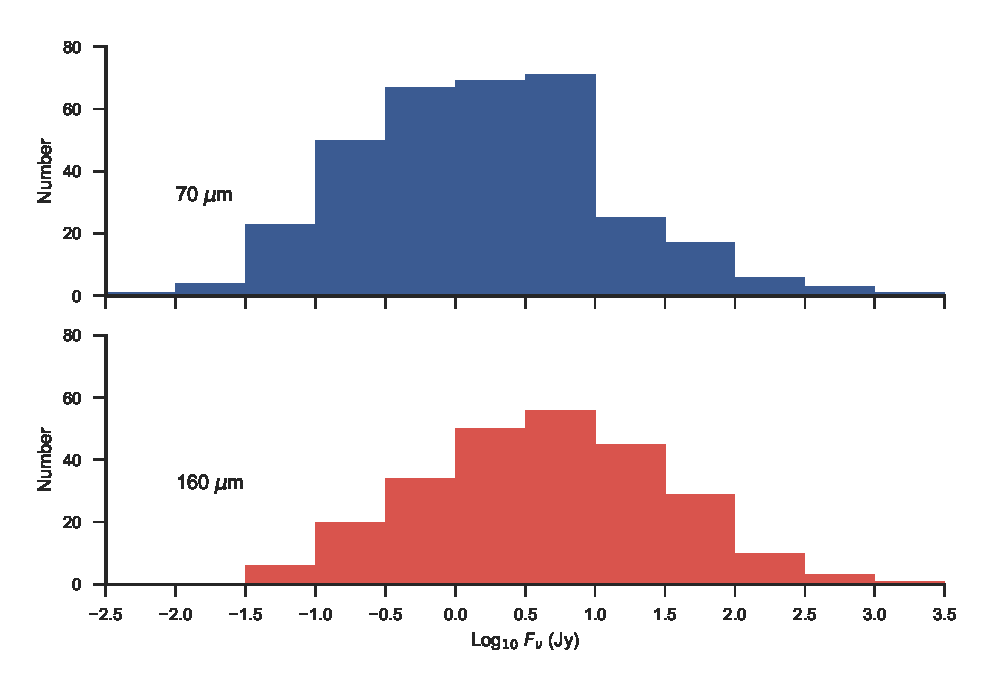
\includegraphics[height=5in]{figures/LFs.eps}
\caption{Flux distributions at 70~\micron\ (top, blue) and 160~\micron\ (bottom, red) for all sources in the HOPS sample.  The upper limits are not used to calculate the distribution.\label{fig:fd}}
\end{figure*}

\begin{figure*}[ht]
\centering
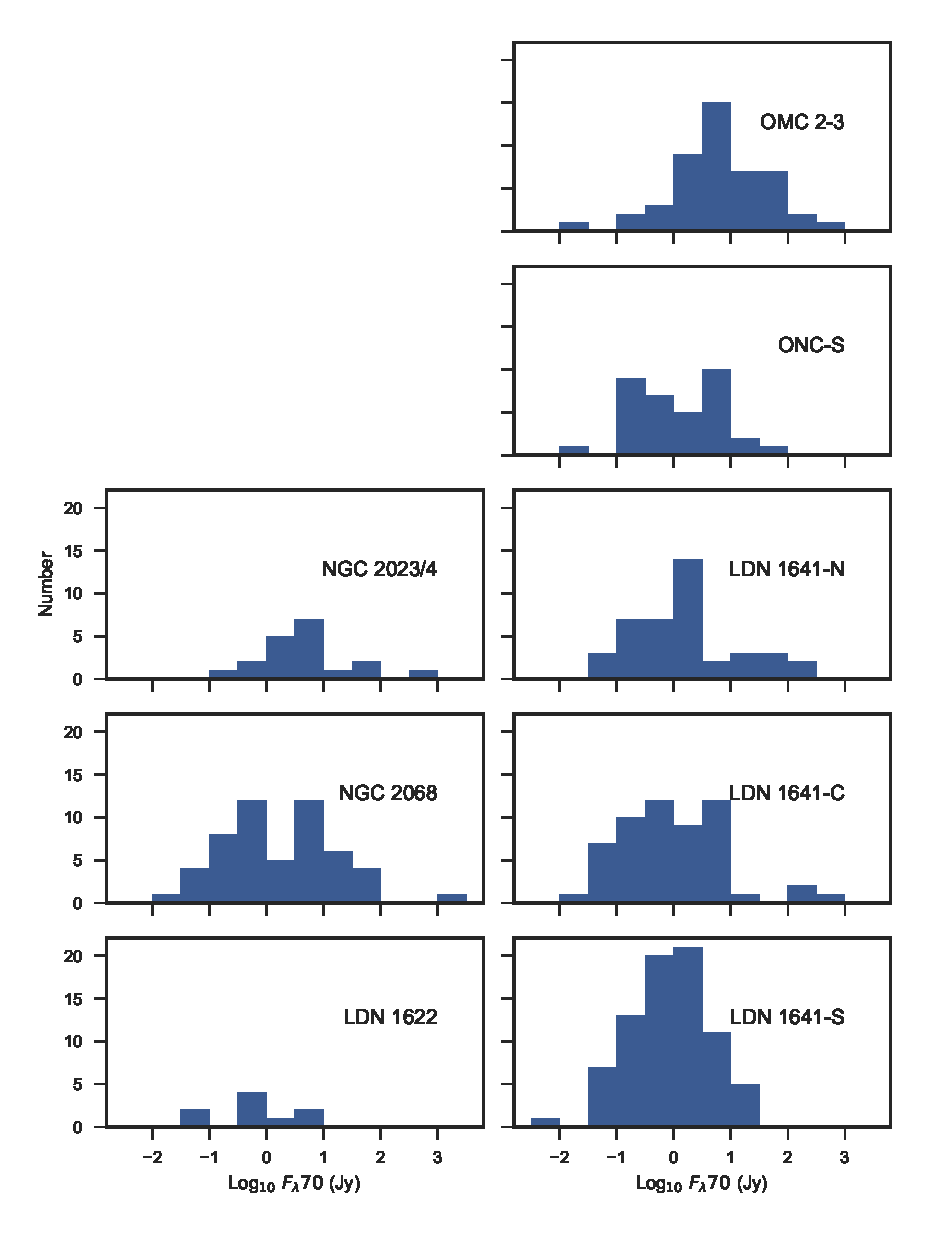
\includegraphics[height=7in]{figures/LF70_byregion.eps}
\caption{The 70\micron\ flux distributions segregated by sub-region for Orion B (left column) and Orion A (right column).\label{fig:fd70regional}}
\end{figure*}

\clearpage

\begin{figure*}[ht]
\centering
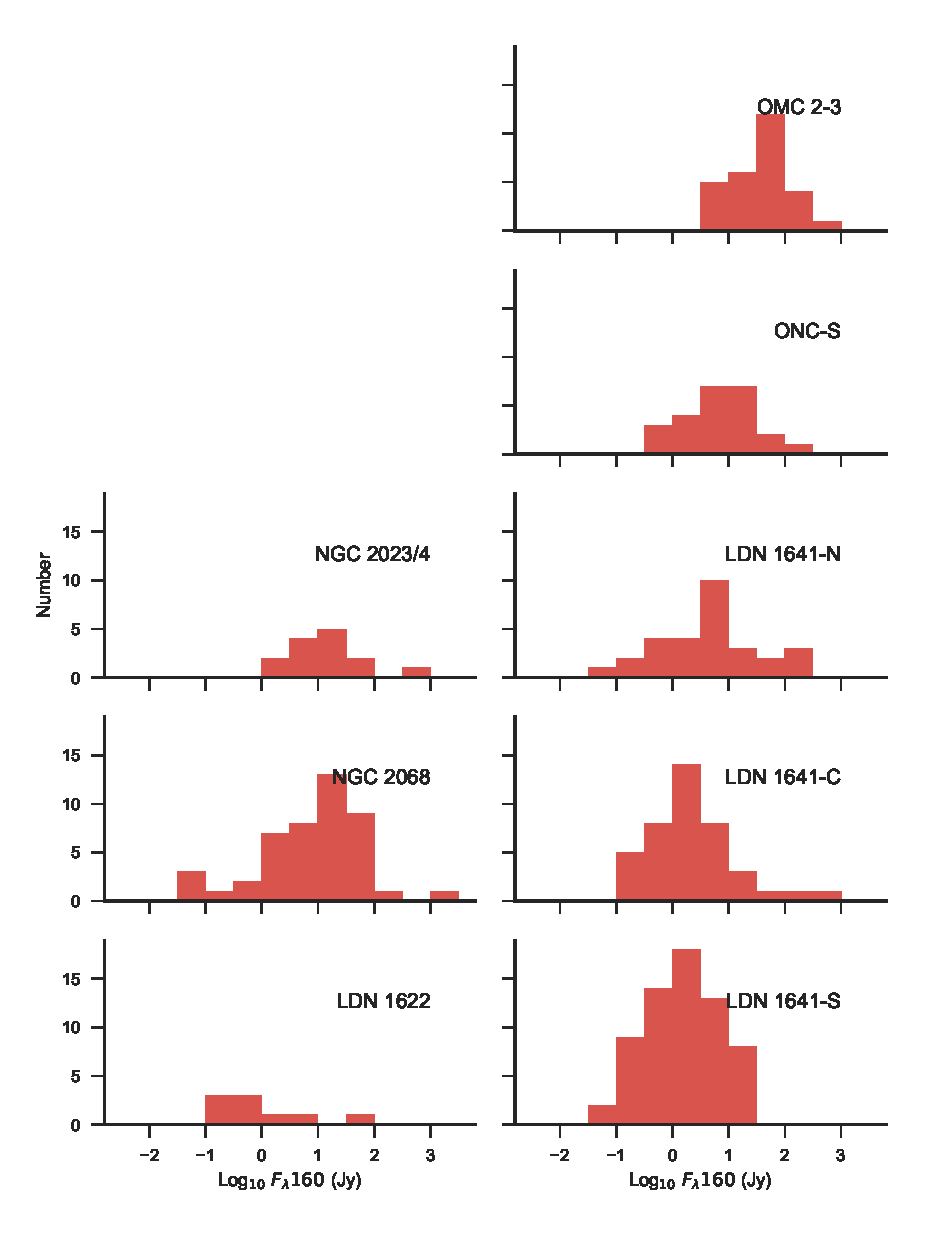
\includegraphics[height=7in]{figures/LF160_byregion.eps}
\caption{The 160\micron\ flux distributions segregated by subregion for Orion B (left column) and Orion A (right column).\label{fig:fd160regional}}
\end{figure*}

\clearpage

\begin{figure*}[ht]
\centering
\plotone{figures/mdFlux_v_dec.eps}
\caption{Median flux as a function of declination for the 70~\micron\ FD (blue dots and curve) and the 160~\micron\ FD (red dots and curve).\label{fig:mdFlux_v_dec}}
\end{figure*}

\clearpage

\begin{figure*}[ht]
\centering
\plotone{figures/OrionA_clrclr.eps}
\caption{The observed distribution of colors in Orion~A segregated by sub-regions.  The sub-region is identified in the respective panel.  Solid red symbols show the colors for the sub-region.  Smaller black open symbols show the distribution for all sources in the combine Orion~A and Orion~B samples.\label{fig:clrclr1}}
\end{figure*}

\clearpage

\begin{figure*}[ht]
\centering
\plotone{figures/OrionB_clrclr.eps}
\caption{Same as Figure~\ref{fig:clrclr1} for Orion~B.\label{fig:clrclr2}}
\end{figure*}

\clearpage

%7
\begin{figure*}[ht]
\centering
\plotone{figures/clr1_vs_dec.eps}
\caption{The mean (black circles) and median (red circles) value of \clra\ color as a function of declination.  The associated sub-region is labelled above the data points themselves.  The vertical bars show the respective standard deviation.  \label{fig:clr1_v_dec}}
\end{figure*}

\clearpage

%8
\begin{figure*}[ht]
\centering
\plotone{figures/clr2_vs_dec.eps}
\caption{Same as Figure~\ref{fig:clr1_v_dec} for the \clrb\ color.  \label{fig:clr2_v_dec}}
\end{figure*}

\clearpage

\begin{figure*}[ht]
\centering
\plotone{figures/num_vs_dec.eps}
\caption{Number of protostars as a function of sub-region in Orion.\label{fig:num_v_dec}}
\end{figure*}

\clearpage

\begin{figure*}[ht]
\centering
\plotone{figures/f70_v_clr2.eps}
\caption{The observed 70~\micron\ flux as a function of the \clra\ (left) and \clrb\ (right) flux ratios.\label{fig:clrflux}}
\end{figure*}

\clearpage

\begin{figure*}[ht]
\centering
\plotone{figures/clr_vs_flimit.png}
\caption{The observed mean color above the simulated completeness limit for LDN~1641.  Solid lines show the mean values for \clra\ (black) and \clrb\ (blue) with limiting flux.  The dashed lines show the mean color for the combined Orion ONC and OMC-2/3 region.  As discussed in text, we note a complete lack of correlation between the completeness limit and mean color for \clrb.  We note a steady increase in the mean \clra as a function of the completeness limit.  However, the average completeness limits require significant differences before the LDN 1641 sub0region can be explained as being similar to Orion OMC-2/3 and the ONC.\label{fig:clr_v_limit}}
\end{figure*}

\appendix

\section{HOPS catalog}
\par
The HOPS observational catalog.
\begin{longrotatetable}
\begin{deluxetable*}{rcccccrcrcrccrc}
\rotate
\tabletypesize{\scriptsize}
\tablecolumns{13}
\tablewidth{0pt}
\tablenum{1}
\tablecaption{The HOPS observation sample\label{tbl:obs}}
\tablehead{
\colhead{HOPS} & 
\colhead{$\alpha_{J2000}$} &
\colhead{$\delta_{J2000}$} &
\colhead{OBSID\tablenotemark{a}} &
\colhead{Group} &
\colhead{$70\mu$m} &
\colhead{flag\tablenotemark{b}} &
\colhead{Method\tablenotemark{c}} &
\colhead{$100\mu$m} &
\colhead{flag\tablenotemark{b}} &
\colhead{$160\mu$m} &
\colhead{flag\tablenotemark{b}} &
\colhead{Method\tablenotemark{c}} &
\colhead{Field} &
\colhead{Observation Date} \\
\colhead{} & 
\colhead{h:m:s} &
\colhead{$^{\rm{o}}:^\prime:^{\prime\prime}$} &
\colhead{} &
\colhead{} &
\colhead{(mJy)} &
\colhead{} &
\colhead{} &
\colhead{(mJy)} &
\colhead{} &
\colhead{(mJy)} &
\colhead{} &
\colhead{} &
\colhead{} &
\colhead{(UT)} \\
\colhead{(1)} & 
\colhead{(2)} &
\colhead{(3)} &
\colhead{(4)} &
\colhead{(5)} &
\colhead{(6)} &
\colhead{(7)} &
\colhead{(8)} &
\colhead{(9)} &
\colhead{(10)} &
\colhead{(11)} &
\colhead{(12)} &
\colhead{(13)} &
\colhead{(14)} &
\colhead{(15)}
}
\startdata
000 &  05:54:28.11 &   01:37:34.9 &  \nodata &  \nodata &  \nodata &  0 &  A &  \nodata &  3 &  \nodata &  0 &  A &  \nodata &  \nodata \\
001 &  05:54:12.34 &   01:42:35.5 &  1342215365-66 &  000 &     3.700 &  1 &  A &     4.570 &  1 &     3.840 &  1 &  A &  LDN 1622        &  6 Mar 2011           \\
002 &  05:54:9.13  &   01:42:52.0 &  1342215365-66 &  000 &     0.519 &  1 &  A &     0.514 &  1 &     0.401 &  1 &  P &  LDN 1622        &  6 Mar 2011           \\
003 &  05:54:56.97 &   01:42:56.2 &  1342218780-81 &  001 &     0.319 &  1 &  A &     0.294 &  1 &     0.262 &  1 &  A &  LDN 1622        &  18 Apr 2011          \\
004 &  05:54:53.76 &   01:47:10.0 &  1342218780-81 &  001 &     0.612 &  1 &  A &     0.622 &  1 &     0.593 &  1 &  A &  LDN 1622        &  18 Apr 2011          \\
005 &  05:54:32.16 &   01:48:7.2  &  1342218703-04 &  003 &     0.710 &  1 &  A &     0.753 &  1 &     0.688 &  1 &  A &  LDN 1622        &  16 Apr 2011          \\
006 &  05:54:18.41 &   01:49:3.4  &  1342218703-04 &  003 &     0.091 &  1 &  A &     0.136 &  1 &     0.190 &  1 &  A &  LDN 1622        &  16 Apr 2011          \\
007 &  05:54:20.04 &   01:50:42.8 &  1342218703-04 &  003 &     1.340 &  1 &  A &     1.750 &  1 &     1.790 &  1 &  A &  LDN 1622        &  16 Apr 2011          \\
008 &  05:35:33.11 &  -05:59:6.4  &  1342227328-29 &  006 &  \nodata &  3 &  A &  \nodata &  3 &  \nodata &  3 &  A &  ONC-S           &  24 Aug 2011          \\
009 &  05:35:49.21 &  -05:59:3.6  &  \nodata &  \nodata &  \nodata &  0 &  A &  \nodata &  3 &  \nodata &  0 &  A &  \nodata &  \nodata \\
010 &  05:35:9.00  &  -05:58:27.6 &  1342204248-49 &  005 &     6.820 &  1 &  A &    12.600 &  1 &    17.700 &  1 &  A &  ONC-S           &  9 Sep 2010           \\
011 &  05:35:13.41 &  -05:57:58.1 &  1342204248-49 &  005 &    23.600 &  1 &  A &    33.000 &  1 &    36.400 &  1 &  A &  ONC-S           &  9 Sep 2010           \\
012 &  05:35:8.60  &  -05:55:54.3 &  1342204248-49 &  005 &    15.600 &  1 &  A &    26.100 &  1 &    41.700 &  1 &  P &  ONC-S           &  9 Sep 2010           \\
013 &  05:35:24.56 &  -05:55:33.4 &  1342227328-29 &  006 &     1.120 &  1 &  A &     0.932 &  1 &     1.070 &  1 &  A &  ONC-S           &  24 Aug 2011          \\
014 &  05:36:19.17 &  -05:55:30.3 &  1342227326-27 &  007 &  \nodata &  3 &  A &  \nodata &  3 &     3.630 &  2 &  A &  ONC-S           &  24 Aug 2011          \\
015 &  05:36:19.02 &  -05:55:25.5 &  1342227326-27 &  007 &     0.258 &  1 &  A &     0.340 &  1 &     2.930 &  2 &  A &  ONC-S           &  24 Aug 2011          \\
016 &  05:35:0.81  &  -05:55:25.7 &  1342204248-49 &  005 &     0.685 &  1 &  A &     1.220 &  1 &     6.470 &  2 &  A &  ONC-S           &  9 Sep 2010           \\
017 &  05:35:7.18  &  -05:52:5.9  &  1342217446-47 &  008 &     0.673 &  1 &  A &     0.541 &  1 &     5.950 &  2 &  A &  ONC-S           &  30 Mar 2011          \\
018 &  05:35:5.49  &  -05:51:54.4 &  1342217446-47 &  008 &     4.270 &  1 &  A &     6.050 &  1 &     6.310 &  1 &  P &  ONC-S           &  30 Mar 2011          \\
019 &  05:35:25.99 &  -05:51:22.9 &  1342217446-47 &  008 &     0.247 &  1 &  A &  \nodata &  3 &     0.953 &  1 &  P &  ONC-S           &  30 Mar 2011          \\
020 &  05:33:30.71 &  -05:50:41.0 &  1342217750-51 &  009 &     1.370 &  1 &  A &     1.710 &  1 &     3.260 &  1 &  A &  ONC-S           &  31 Mar 2011          \\
021 &  05:36:10.10 &  -05:50:8.3  &  1342227096-97 &  010 &     0.119 &  1 &  A &     0.299 &  2 &     1.380 &  2 &  A &  ONC-S           &  22 Aug 2011          \\
022 &  05:35:0.53  &  -05:49:2.0  &  1342217446-47 &  008 &     0.146 &  1 &  A &     0.550 &  2 &     6.370 &  2 &  A &  ONC-S           &  30 Mar 2011          \\
023 &  05:36:17.89 &  -05:46:54.5 &  1342227096-97 &  010 &  \nodata &  3 &  A &  \nodata &  3 &  \nodata &  3 &  A &  ONC-S           &  22 Aug 2011          \\
024 &  05:34:46.94 &  -05:44:51.0 &  1342204246-47 &  012 &     0.291 &  1 &  A &  \nodata &  3 &     0.581 &  2 &  A &  ONC-S           &  9 Sep 2010           \\
025 &  05:35:22.63 &  -05:44:29.5 &  1342227098-99 &  013 &  \nodata &  3 &  A &  \nodata &  3 &  \nodata &  3 &  A &  ONC-S           &  22 Aug 2011          \\
026 &  05:35:17.34 &  -05:42:14.5 &  1342227098-99 &  013 &     0.130 &  1 &  A &  \nodata &  3 &     2.300 &  2 &  A &  ONC-S           &  22 Aug 2011          \\
027 &  05:36:21.72 &  -05:41:58.1 &  \nodata &  \nodata &  \nodata &  0 &  A &     0.493 &  1 &  \nodata &  0 &  A &  \nodata &  \nodata \\
028 &  05:34:47.29 &  -05:41:55.9 &  1342204246-47 &  012 &     0.945 &  1 &  A &     1.850 &  1 &     2.570 &  1 &  P &  ONC-S           &  9 Sep 2010           \\
029 &  05:34:49.04 &  -05:41:42.2 &  1342204246-47 &  012 &     3.770 &  1 &  A &     4.120 &  1 &     3.900 &  1 &  P &  ONC-S           &  9 Sep 2010           \\
030 &  05:34:44.06 &  -05:41:25.9 &  1342204246-47 &  012 &     7.610 &  1 &  A &     9.370 &  1 &    13.000 &  1 &  P &  ONC-S           &  9 Sep 2010           \\
031 &  05:35:17.25 &  -05:40:26.9 &  1342227098-99 &  013 &  \nodata &  3 &  A &  \nodata &  3 &  \nodata &  3 &  A &  ONC-S           &  22 Aug 2011          \\
032 &  05:34:35.45 &  -05:39:59.1 &  1342204244-45 &  014 &     6.170 &  1 &  A &     5.550 &  1 &     7.710 &  1 &  P &  ONC-S           &  9 Sep 2010           \\
033 &  05:34:45.21 &  -05:39:56.8 &  1342204246-47 &  012 &     0.108 &  1 &  A &  \nodata &  3 &     0.751 &  2 &  A &  ONC-S           &  9 Sep 2010           \\
034 &  05:35:10.90 &  -05:39:30.7 &  1342205234-35 &  015 &  \nodata & 3 &  A &  \nodata &  3 &  \nodata &  3 &  A &  ONC-S           &  28 Sep 2010          \\
035 &  05:35:19.93 &  -05:39:1.2  &  1342205234-35 &  015 &  \nodata &  3 &  A &  \nodata &  3 &  \nodata &  3 &  A &  ONC-S           &  28 Sep 2010          \\
036 &  05:34:26.43 &  -05:37:40.5 &  1342204244-45 &  014 &     0.997 &  1 &  A &     1.020 &  1 &     0.872 &  1 &  A &  ONC-S           &  9 Sep 2010           \\
037 &  05:34:47.67 &  -05:37:25.2 &  1342204244-45 &  014 &  \nodata &  3 &  A &  \nodata &  3 &  \nodata &  3 &  A &  ONC-S           &  9 Sep 2010           \\
038 &  05:35:4.72  &  -05:37:12.3 &  1342205234-35 &  015 &     0.272 &  1 &  P &  \nodata &  3 &    17.000 &  2 &  A &  ONC-S           &  28 Sep 2010          \\
039 &  05:36:22.43 &  -05:36:24.8 &  \nodata &  \nodata &  \nodata &  0 &  A &     0.445 &  1 &  \nodata &  0 &  A &  \nodata &  \nodata \\
040 &  05:35:8.52  &  -05:35:59.4 &  1342205234-35 &  015 &     3.310 &  1 &  A &    11.600 &  1 &    14.600 &  1 &  P &  ONC-S           &  28 Sep 2010          \\
041 &  05:34:29.44 &  -05:35:42.7 &  1342204244-45 &  014 &     4.560 &  1 &  A &     7.040 &  1 &    10.600 &  1 &  A &  ONC-S           &  9 Sep 2010           \\
042 &  05:35:5.04  &  -05:35:40.7 &  1342205234-35 &  015 &     1.310 &  1 &  A &  \nodata &  3 &    28.800 &  2 &  A &  ONC-S           &  28 Sep 2010          \\
043 &  05:35:4.50  &  -05:35:14.4 &  1342205234-35 &  015 &     3.250 &  1 &  P &    14.700 &  1 &    17.200 &  1 &  P &  ONC-S           &  28 Sep 2010          \\
044 &  05:35:10.57 &  -05:35:6.3  &  1342205234-35 &  015 &     0.956 &  1 &  P &  \nodata &  3 &    13.000 &  1 &  A &  ONC-S           &  28 Sep 2010          \\
045 &  05:35:6.45  &  -05:33:35.1 &  1342205234-35 &  015 &     6.550 &  1 &  P &  \nodata &  3 &     8.530 &  1 &  A &  ONC-S           &  28 Sep 2010          \\
046 &  05:34:42.20 &  -05:33:3.3  &  1342217448-49 &  016 &  \nodata &  3 &  A &  \nodata &  3 &     6.330 &  2 &  A &  ONC-S           &  30 Mar 2011          \\
047 &  05:33:45.87 &  -05:32:58.1 &  1342204433-34 &  308 &     0.018 &  1 &  A &  \nodata &  3 &     0.490 &  2 &  A &  ONC-S           &  13 Sep 2010          \\
048 &  05:35:6.56  &  -05:32:51.6 &  1342205234-35 &  015 &     5.670 &  2 &  A &  \nodata &  3 &  \nodata &  3 &  A &  ONC-S           &  28 Sep 2010          \\
049 &  05:34:48.88 &  -05:31:45.9 &  1342217448-49 &  016 &     0.664 &  1 &  A &  \nodata &  3 &     0.622 &  2 &  A &  ONC-S           &  30 Mar 2011          \\
050 &  05:34:40.91 &  -05:31:44.4 &  1342217448-49 &  016 &     9.110 &  1 &  A &    14.200 &  1 &    20.300 &  1 &  A &  ONC-S           &  30 Mar 2011          \\
051 &  05:35:15.83 &  -05:30:5.5  &  1342217450-51 &  017 &  \nodata &  3 &  A &  \nodata &  3 &  \nodata &  3 &  A &  ONC-S           &  30 Mar 2011          \\
052 &  05:35:16.32 &  -05:29:32.6 &  1342217450-51 &  017 &  \nodata &  3 &  A &  \nodata &  3 &  \nodata &  3 &  A &  ONC-S           &  30 Mar 2011          \\
053 &  05:33:57.37 &  -05:23:30.4 &  1342217752-53 &  018 &    69.000 &  1 &  A &   106.000 &  1 &   103.000 &  1 &  A &  ONC-S           &  31 Mar 2011          \\
054 &  05:33:22.48 &  -05:23:2.9  &  \nodata &  \nodata &  \nodata &  0 &  A &  \nodata &  3 &  \nodata &  0 &  A &  \nodata &  \nodata \\
055 &  05:33:54.09 &  -05:21:49.5 &  1342217752-53 &  018 &  \nodata &  3 &  A &  \nodata &  3 &     1.230 &  1 &  A &  ONC-S           &  31 Mar 2011          \\
056 &  05:35:19.47 &  -05:15:32.7 &  1342205232-33 &  200 &    47.200 &  1 &  A &    94.100 &  1 &   128.000 &  1 &  P &  OMC 2-3         &  28 Sep 2010          \\
057 &  05:35:19.84 &  -05:15:8.5  &  1342205232-33 &  200 &     4.910 &  1 &  A &  \nodata &  3 &    75.100 &  2 &  A &  OMC 2-3         &  28 Sep 2010          \\
058 &  05:35:18.51 &  -05:13:38.2 &  1342205232-33 &  200 &     3.460 &  1 &  A &  \nodata &  3 &     3.810 &  2 &  A &  OMC 2-3         &  28 Sep 2010          \\
059 &  05:35:20.14 &  -05:13:15.5 &  1342205232-33 &  200 &    58.400 &  1 &  A &    65.600 &  1 &    58.100 &  1 &  P &  OMC 2-3         &  28 Sep 2010          \\
060 &  05:35:23.33 &  -05:12:3.1  &  1342205228-29 &  130 &    58.300 &  1 &  A &    83.400 &  1 &    84.600 &  1 &  A &  OMC 2-3         &  28 Sep 2010          \\
061 &  05:33:25.91 &  -05:12:2.6  &  \nodata &  \nodata &  \nodata &  0 &  A &  \nodata &  3 &  \nodata &  0 &  A &  \nodata &  \nodata \\
062 &  05:35:24.58 &  -05:11:29.7 &  1342205228-29 &  130 &  \nodata &  3 &  A &  \nodata &  3 &    44.000 &  2 &  A &  OMC 2-3         &  28 Sep 2010          \\
063 &  05:35:24.90 &  -05:10:1.5  &  1342205228-29 &  130 &  \nodata &  3 &  A &  \nodata &  3 &  \nodata &  3 &  A &  OMC 2-3         &  28 Sep 2010          \\
064 &  05:35:27.00 &  -05:09:54.1 &  1342205228-29 &  130 &  \nodata &  3 &  A &  \nodata &  3 &  \nodata &  3 &  A &  OMC 2-3         &  28 Sep 2010          \\
065 &  05:35:21.55 &  -05:09:38.7 &  1342205228-29 &  130 &     0.481 &  1 &  A &  \nodata &  3 &    28.400 &  2 &  A &  OMC 2-3         &  28 Sep 2010          \\
066 &  05:35:26.84 &  -05:09:24.6 &  1342205228-29 &  130 &    27.200 &  1 &  P &  \nodata &  3 &   325.000 &  2 &  A &  OMC 2-3         &  28 Sep 2010          \\
067 &  05:35:22.69 &  -05:08:34.0 &  1342205228-29 &  130 &  \nodata &  3 &  A &  \nodata &  3 &  \nodata &  3 &  A &  OMC 2-3         &  28 Sep 2010          \\
068 &  05:35:24.30 &  -05:08:30.6 &  1342205228-29 &  130 &     6.960 &  1 &  A &    14.300 &  1 &    25.500 &  1 &  A &  OMC 2-3         &  28 Sep 2010          \\
069 &  05:35:25.22 &  -05:08:24.0 &  1342205228-29 &  130 &  \nodata &  3 &  A &  \nodata &  3 &    15.600 &  2 &  A &  OMC 2-3         &  28 Sep 2010          \\
070 &  05:35:22.41 &  -05:08:4.8  &  1342205228-29 &  130 &     6.410 &  1 &  P &  \nodata &  3 &    11.600 &  1 &  A &  OMC 2-3         &  28 Sep 2010          \\
071 &  05:35:25.61 &  -05:07:57.3 &  1342205228-29 &  130 &    14.300 &  1 &  A &    13.100 &  1 &    46.800 &  2 &  A &  OMC 2-3         &  28 Sep 2010          \\
072 &  05:35:25.71 &  -05:07:46.4 &  1342205228-29 &  130 &  \nodata &  3 &  A &  \nodata &  3 &  \nodata &  3 &  A &  OMC 2-3         &  28 Sep 2010          \\
073 &  05:35:27.70 &  -05:07:3.5  &  1342205226-27 &  135 &     1.670 &  1 &  A &     7.110 &  1 &    11.700 &  1 &  A &  OMC 2-3         &  28 Sep 2010          \\
074 &  05:35:24.86 &  -05:06:21.4 &  1342205228-29 &  130 &     1.010 &  1 &  A &  \nodata &  3 &    23.800 &  2 &  A &  OMC 2-3         &  28 Sep 2010          \\
075 &  05:35:26.66 &  -05:06:10.3 &  1342205226-27 &  135 &     7.030 &  1 &  A &    11.900 &  1 &    21.900 &  1 &  P &  OMC 2-3         &  28 Sep 2010          \\
076 &  05:35:25.75 &  -05:05:57.9 &  1342205226-27 &  135 &     2.160 &  1 &  P &  \nodata &  3 &     9.740 &  1 &  A &  OMC 2-3         &  28 Sep 2010          \\
077 &  05:35:31.53 &  -05:05:47.3 &  1342205226-27 &  135 &     8.870 &  1 &  A &     9.090 &  1 &    34.000 &  2 &  A &  OMC 2-3         &  28 Sep 2010          \\
078 &  05:35:25.82 &  -05:05:43.7 &  1342205226-27 &  135 &    15.100 &  1 &  A &    35.500 &  1 &    56.700 &  1 &  P &  OMC 2-3         &  28 Sep 2010          \\
079 &  05:35:27.88 &  -05:05:36.3 &  1342205228-29 &  130 &  \nodata &  3 &  A &  \nodata &  3 &  \nodata &  3 &  A &  OMC 2-3         &  28 Sep 2010          \\
080 &  05:35:25.19 &  -05:05:9.5  &  1342205226-27 &  135 &     0.155 &  1 &  A &  \nodata &  3 &  \nodata &  3 &  A &  OMC 2-3         &  28 Sep 2010          \\
081 &  05:35:27.95 &  -05:04:58.2 &  1342205226-27 &  135 &     1.990 &  1 &  A &     4.030 &  1 &     8.240 &  1 &  A &  OMC 2-3         &  28 Sep 2010          \\
082 &  05:35:19.73 &  -05:04:54.6 &  1342205226-27 &  135 &     3.780 &  1 &  P &     7.280 &  1 &    10.400 &  1 &  A &  OMC 2-3         &  28 Sep 2010          \\
083 &  05:35:55.73 &  -05:04:37.6 &  \nodata &  \nodata &  \nodata &  0 &  A &  \nodata &  3 &  \nodata &  0 &  A &  \nodata &  \nodata \\
084 &  05:35:26.57 &  -05:03:55.1 &  1342205226-27 &  135 &   104.000 &  1 &  A &   117.000 &  1 &   132.000 &  1 &  A &  OMC 2-3         &  28 Sep 2010          \\
085 &  05:35:28.18 &  -05:03:40.9 &  1342205226-27 &  135 &    29.000 &  1 &  A &    36.000 &  1 &    48.000 &  1 &  P &  OMC 2-3         &  28 Sep 2010          \\
086 &  05:35:23.65 &  -05:01:40.3 &  1342204250-51 &  019 &     6.100 &  1 &  P &    86.500 &  2 &    19.300 &  2 &  A &  OMC 2-3         &  10 Sep 2010          \\
087 &  05:35:23.47 &  -05:01:28.7 &  1342204250-51 &  019 &    63.600 &  1 &  P &   158.000 &  1 &   230.000 &  1 &  P &  OMC 2-3         &  10 Sep 2010          \\
088 &  05:35:22.43 &  -05:01:14.2 &  1342204250-51 &  019 &    32.800 &  1 &  A &    69.500 &  1 &    81.600 &  1 &  P &  OMC 2-3         &  10 Sep 2010          \\
089 &  05:35:19.96 &  -05:01:2.6  &  1342204250-51 &  019 &     3.340 &  1 &  A &  \nodata &  3 &    29.600 &  2 &  A &  OMC 2-3         &  10 Sep 2010          \\
090 &  05:35:34.47 &  -05:00:52.0 &  1342204250-51 &  019 &     2.370 &  1 &  A &     1.780 &  1 &     0.416 &  2 &  A &  OMC 2-3         &  10 Sep 2010          \\
091 &  05:35:18.91 &  -05:00:50.9 &  1342204250-51 &  019 &     3.350 &  1 &  P &    15.800 &  1 &    34.300 &  1 &  P &  OMC 2-3         &  10 Sep 2010          \\
092 &  05:35:18.32 &  -05:00:33.0 &  1342204250-51 &  019 &    33.000 &  1 &  A &    51.000 &  1 &    56.200 &  1 &  P &  OMC 2-3         &  10 Sep 2010          \\
093 &  05:35:15.03 &  -05:00:8.2  &  1342204250-51 &  019 &     2.490 &  1 &  A &  \nodata &  3 &    49.000 &  2 &  A &  OMC 2-3         &  10 Sep 2010          \\
094 &  05:35:16.15 &  -05:00:2.3  &  1342204250-51 &  019 &     6.340 &  1 &  A &    18.000 &  1 &    32.800 &  1 &  P &  OMC 2-3         &  10 Sep 2010          \\
095 &  05:35:34.20 &  -04:59:52.2 &  1342204250-51 &  019 &     0.632 &  1 &  P &     2.420 &  1 &     5.900 &  1 &  P &  OMC 2-3         &  10 Sep 2010          \\
096 &  05:35:29.72 &  -04:58:48.8 &  1342204250-51 &  019 &     6.900 &  1 &  A &    20.100 &  1 &    51.200 &  1 &  A &  OMC 2-3         &  10 Sep 2010          \\
097 &  05:35:28.89 &  -04:57:38.9 &  1342204250-51 &  019 &  \nodata &  3 &  A &  \nodata &  3 &  \nodata &  3 &  A &  OMC 2-3         &  10 Sep 2010          \\
098 &  05:35:19.32 &  -04:55:44.9 &  1342204250-51 &  019 &     1.650 &  1 &  P &  \nodata &  3 &     4.640 &  2 &  A &  OMC 2-3         &  10 Sep 2010          \\
099 &  05:34:29.50 &  -04:55:30.6 &  1342217754-55 &  021 &     3.600 &  1 &  A &     6.190 &  1 &     8.850 &  1 &  A &  OMC 2-3         &  31 Mar 2011          \\
100 &  05:34:21.39 &  -04:55:14.8 &  1342217754-55 &  021 &     0.015 &  1 &  A &  \nodata &  3 &     2.330 &  2 &  A &  OMC 2-3         &  31 Mar 2011          \\
101 &  05:35:8.22  &  -04:54:9.7  &  1342217758-59 &  020 &     2.840 &  1 &  A &  \nodata &  3 &    48.100 &  2 &  A &  OMC 2-3         &  31 Mar 2011          \\
102 &  05:34:35.18 &  -04:52:17.9 &  1342217754-55 &  021 &     0.640 &  1 &  A &     0.693 &  1 &     4.680 &  2 &  A &  OMC 2-3         &  31 Mar 2011          \\
103 &  05:34:12.19 &  -04:50:7.0  &  1342217754-55 &  021 &  \nodata &  3 &  A &  \nodata &  3 &  \nodata &  3 &  A &  OMC 2-3         &  31 Mar 2011          \\
104 &  05:35:6.78  &  -04:50:1.8  &  1342217758-59 &  020 &  \nodata &  3 &  A &  \nodata &  3 &  \nodata &  3 &  A &  OMC 2-3         &  31 Mar 2011          \\
105 &  05:35:32.28 &  -04:46:48.5 &  1342191970-71 &  306 &     0.259 &  1 &  A &  \nodata &  3 &     1.130 &  2 &  A &  OMC 2-3         &  10 Mar 2010          \\
106 &  05:36:12.43 &  -04:45:15.7 &  \nodata &  \nodata &  \nodata &  0 &  A &  \nodata &  3 &  \nodata &  0 &  A &  \nodata &  \nodata \\
107 &  05:35:23.34 &  -04:40:10.5 &  1342217756-57 &  024 &     4.370 &  1 &  A &     5.060 &  1 &     5.560 &  1 &  A &  OMC 2-3         &  31 Mar 2011          \\
108 &  05:35:27.07 &  -05:10:0.4  &  1342205228-29 &  130 &    40.800 &  1 &  P &   288.000 &  2 &   270.000 &  1 &  P &  OMC 2-3         &  28 Sep 2010          \\
109 &  05:35:8.56  &  -05:35:59.2 &  1342205234-35 &  015 &  \nodata &  0 &  A &  \nodata &  0 &  \nodata &  0 &  A &  ONC-S           &  28 Sep 2010          \\
110 &  05:36:2.23  &  -05:02:49.8 &  \nodata &  \nodata &  \nodata &  0 &  A &  \nodata &  3 &  \nodata &  0 &  A &  \nodata &  \nodata \\
111 &  05:35:23.36 &  -05:12:2.8  &  1342205226-27 &  135 &  \nodata &  0 &  A &  \nodata &  0 &  \nodata &  0 &  A &  OMC 2-3         &  28 Sep 2010          \\
112 &  05:40:43.99 &  -07:22:42.9 &  \nodata &  \nodata &  \nodata &  0 &  A &  \nodata &  3 &  \nodata &  0 &  A &  \nodata &  \nodata \\
113 &  05:39:58.13 &  -07:26:41.2 &  1342215589-90 &  025 &     0.059 &  1 &  A &  \nodata &  3 &     0.256 &  2 &  A &  LDN 1641-C      &  7 Mar 2011           \\
114 &  05:40:1.37  &  -07:25:38.6 &  1342215589-90 &  025 &     0.111 &  1 &  A &     0.140 &  1 &     0.124 &  2 &  A &  LDN 1641-C      &  7 Mar 2011           \\
115 &  05:39:56.50 &  -07:25:51.5 &  1342215589-90 &  025 &     0.260 &  1 &  A &     0.287 &  1 &     0.258 &  1 &  P &  LDN 1641-C      &  7 Mar 2011           \\
116 &  05:39:57.90 &  -07:25:13.1 &  1342215589-90 &  025 &     0.328 &  1 &  A &     0.302 &  1 &     0.398 &  1 &  P &  LDN 1641-C      &  7 Mar 2011           \\
117 &  05:39:55.44 &  -07:24:19.5 &  1342215589-90 &  025 &     0.123 &  1 &  A &     0.179 &  1 &     0.243 &  1 &  P &  LDN 1641-C      &  7 Mar 2011           \\
118 &  05:39:54.58 &  -07:24:14.8 &  1342215589-90 &  025 &     0.129 &  1 &  A &     0.073 &  1 &     0.078 &  2 &  A &  LDN 1641-C      &  7 Mar 2011           \\
119 &  05:39:50.65 &  -07:23:30.4 &  1342215589-90 &  025 &     0.746 &  1 &  A &     0.682 &  1 &     0.578 &  1 &  P &  LDN 1641-C      &  7 Mar 2011           \\
120 &  05:39:34.32 &  -07:26:11.4 &  1342218729-30 &  026 &     0.162 &  1 &  A &     0.169 &  1 &     0.539 &  1 &  P &  LDN 1641-C      &  17 Apr 2011          \\
121 &  05:39:33.70 &  -07:23:2.0  &  1342227084-85 &  313 &     0.427 &  1 &  A &     1.260 &  1 &     2.880 &  2 &  A &  LDN 1641-C      &  22 Aug 2011          \\
122 &  05:39:45.13 &  -07:19:13.5 &  1342215589-90 &  025 &     0.045 &  1 &  A &  \nodata &  3 &  \nodata &  3 &  A &  LDN 1641-C      &  7 Mar 2011           \\
123 &  05:39:33.30 &  -07:22:57.4 &  1342227084-85 &  313 &     0.614 &  1 &  A &     1.260 &  1 &     2.470 &  1 &  A &  LDN 1641-C      &  22 Aug 2011          \\
124 &  05:39:19.98 &  -07:26:11.2 &  1342218729-30 &  026 &   165.000 &  1 &  A &   233.000 &  1 &   236.000 &  1 &  A &  LDN 1641-C      &  17 Apr 2011          \\
125 &  05:39:19.61 &  -07:26:18.8 &  1342218729-30 &  026 &    21.600 &  1 &  P &   233.000 &  2 &  \nodata &  3 &  A &  LDN 1641-C      &  17 Apr 2011          \\
126 &  05:40:9.80  &  -07:09:53.9 &  \nodata &  \nodata &  \nodata &  0 &  A &  \nodata &  3 &  \nodata &  0 &  A &  \nodata &  \nodata \\
127 &  05:39:0.94  &  -07:20:22.6 &  1342227086-87 &  028 &     0.754 &  1 &  A &     0.872 &  1 &     1.270 &  1 &  A &  LDN 1641-C      &  22 Aug 2011          \\
128 &  05:38:52.01 &  -07:21:6.0  &  1342227086-87 &  028 &     0.398 &  1 &  P &     0.738 &  1 &     0.517 &  1 &  P &  LDN 1641-C      &  22 Aug 2011          \\
129 &  05:39:11.85 &  -07:10:35.0 &  1342204252-53 &  029 &     3.490 &  1 &  A &     4.920 &  1 &     4.270 &  1 &  P &  LDN 1641-C      &  10 Sep 2010          \\
130 &  05:39:2.96  &  -07:12:52.3 &  1342204252-53 &  029 &     2.170 &  1 &  A &     2.930 &  1 &     2.450 &  1 &  A &  LDN 1641-C      &  10 Sep 2010          \\
131 &  05:39:7.57  &  -07:10:52.1 &  1342204252-53 &  029 &     0.386 &  1 &  A &     0.459 &  1 &     0.489 &  1 &  A &  LDN 1641-C      &  10 Sep 2010          \\
132 &  05:39:5.36  &  -07:11:5.2  &  1342204252-53 &  029 &     0.678 &  1 &  A &     0.562 &  1 &     0.667 &  1 &  A &  LDN 1641-C      &  10 Sep 2010          \\
133 &  05:39:5.83  &  -07:10:39.4 &  1342204252-53 &  029 &     6.980 &  1 &  A &     8.280 &  1 &     9.370 &  1 &  A &  LDN 1641-C      &  10 Sep 2010          \\
134 &  05:38:42.78 &  -07:12:43.8 &  1342204254-55 &  030 &     3.450 &  1 &  A &     3.580 &  1 &     3.290 &  1 &  A &  LDN 1641-C      &  10 Sep 2010          \\
135 &  05:38:45.31 &  -07:10:55.9 &  1342204254-55 &  030 &     2.360 &  1 &  A &     2.490 &  1 &     2.530 &  1 &  A &  LDN 1641-C      &  10 Sep 2010          \\
136 &  05:38:46.54 &  -07:05:37.5 &  1342205242-43 &  312 &     1.670 &  1 &  A &     2.030 &  1 &     2.110 &  1 &  P &  LDN 1641-C      &  28 Sep 2010          \\
137 &  05:38:53.95 &  -07:02:33.2 &  1342204256-57 &  031 &     0.037 &  1 &  A &  \nodata &  3 &     0.202 &  2 &  A &  LDN 1641-C      &  10 Sep 2010          \\
138 &  05:38:48.33 &  -07:02:43.4 &  1342205242-43 &  312 &     0.052 &  1 &  A &  \nodata &  3 &     1.350 &  2 &  A &  LDN 1641-C      &  28 Sep 2010          \\
139 &  05:38:49.62 &  -07:01:17.8 &  1342204256-57 &  031 &     6.450 &  1 &  A &     6.250 &  1 &     7.360 &  1 &  A &  LDN 1641-C      &  10 Sep 2010          \\
140 &  05:38:46.28 &  -07:01:53.5 &  1342204256-57 &  031 &     1.120 &  1 &  A &     1.450 &  1 &     1.940 &  1 &  P &  LDN 1641-C      &  10 Sep 2010          \\
141 &  05:38:48.01 &  -07:00:49.5 &  1342204256-57 &  031 &     0.104 &  1 &  A &  \nodata &  3 &     0.307 &  2 &  A &  LDN 1641-C      &  10 Sep 2010          \\
142 &  05:38:47.77 &  -07:00:26.9 &  1342204256-57 &  031 &     0.074 &  1 &  A &  \nodata &  3 &     0.985 &  2 &  A &  LDN 1641-C      &  10 Sep 2010          \\
143 &  05:38:46.19 &  -07:00:48.6 &  1342204256-57 &  031 &     5.390 &  1 &  A &     6.500 &  1 &     6.900 &  1 &  A &  LDN 1641-C      &  10 Sep 2010          \\
144 &  05:38:45.01 &  -07:01:1.7  &  1342204256-57 &  031 &     4.840 &  1 &  P &    13.400 &  2 &    13.600 &  2 &  A &  LDN 1641-C      &  10 Sep 2010          \\
145 &  05:38:43.84 &  -07:01:13.2 &  1342204256-57 &  031 &     4.300 &  1 &  A &     3.940 &  1 &     2.700 &  1 &  P &  LDN 1641-C      &  10 Sep 2010          \\
146 &  05:38:44.16 &  -07:00:40.4 &  1342204256-57 &  031 &  \nodata &  3 &  A &  \nodata &  3 &     3.470 &  2 &  A &  LDN 1641-C      &  10 Sep 2010          \\
147 &  05:38:55.00 &  -06:56:18.6 &  1342204256-57 &  031 &     0.045 &  1 &  A &  \nodata &  3 &     0.032 &  2 &  A &  LDN 1641-C      &  10 Sep 2010          \\
148 &  05:38:39.51 &  -06:59:30.3 &  1342204256-57 &  031 &     0.553 &  1 &  A &     0.466 &  1 &     0.419 &  1 &  P &  LDN 1641-C      &  10 Sep 2010          \\
149 &  05:38:40.48 &  -06:58:21.7 &  1342204256-57 &  031 &     7.770 &  1 &  A &     7.550 &  1 &     5.880 &  1 &  A &  LDN 1641-C      &  10 Sep 2010          \\
150 &  05:38:7.53  &  -07:08:29.2 &  1342227045-46 &  032 &     6.180 &  1 &  A &     7.410 &  1 &     9.580 &  1 &  A &  LDN 1641-C      &  21 Aug 2011          \\
151 &  05:38:42.88 &  -06:56:40.7 &  1342204256-57 &  031 &  \nodata &  3 &  A &  \nodata &  3 &  \nodata &  3 &  A &  LDN 1641-C      &  10 Sep 2010          \\
152 &  05:37:58.76 &  -07:07:25.3 &  1342227045-46 &  032 &     1.330 &  1 &  A &     1.860 &  1 &     3.140 &  1 &  P &  LDN 1641-C      &  21 Aug 2011          \\
153 &  05:37:57.01 &  -07:06:56.5 &  1342227045-46 &  032 &     7.250 &  1 &  A &    17.000 &  1 &    29.600 &  1 &  A &  LDN 1641-C      &  21 Aug 2011          \\
154 &  05:38:20.09 &  -06:59:4.8  &  1342228171-72 &  033 &     0.167 &  1 &  A &     0.150 &  1 &     0.163 &  1 &  A &  LDN 1641-C      &  4 Sep 2011           \\
155 &  05:37:15.84 &  -07:17:50.0 &  \nodata &  \nodata &  \nodata &  0 &  A &  \nodata &  3 &  \nodata &  0 &  A &  \nodata &  \nodata \\
156 &  05:38:3.40  &  -06:58:15.8 &  1342205240-41 &  034 &     0.673 &  1 &  A &     0.773 &  1 &     1.050 &  1 &  P &  LDN 1641-C      &  28 Sep 2010          \\
157 &  05:37:56.57 &  -06:56:39.2 &  1342205240-41 &  034 &     7.620 &  1 &  A &    11.400 &  1 &    11.100 &  1 &  A &  LDN 1641-C      &  28 Sep 2010          \\
158 &  05:37:24.46 &  -06:58:32.8 &  1342227314-15 &  035 &     1.450 &  1 &  A &     1.400 &  1 &     1.480 &  1 &  P &  LDN 1641-C      &  24 Aug 2011          \\
159 &  05:37:53.74 &  -06:47:16.9 &  1342227088-89 &  036 &     0.227 &  1 &  A &     0.216 &  1 &     0.161 &  1 &  A &  LDN 1641-N      &  22 Aug 2011          \\
160 &  05:37:51.04 &  -06:47:20.4 &  1342227088-89 &  036 &     2.850 &  1 &  A &     4.110 &  1 &     3.860 &  1 &  P &  LDN 1641-N      &  22 Aug 2011          \\
161 &  05:36:34.76 &  -07:11:13.7 &  \nodata &  \nodata &  \nodata &  0 &  A &     0.231 &  1 &  \nodata &  0 &  A &  \nodata &  \nodata \\
162 &  05:36:30.97 &  -06:52:40.9 &  \nodata &  \nodata &  \nodata &  0 &  A &  \nodata &  3 &  \nodata &  0 &  A &  \nodata &  \nodata \\
163 &  05:37:17.28 &  -06:36:18.2 &  1342227090-91 &  037 &     0.878 &  1 &  A &     0.721 &  1 &     0.765 &  1 &  A &  LDN 1641-N      &  22 Aug 2011          \\
164 &  05:37:0.45  &  -06:37:10.5 &  1342227090-91 &  037 &     0.738 &  1 &  A &     1.720 &  1 &     4.100 &  1 &  A &  LDN 1641-N      &  22 Aug 2011          \\
165 &  05:36:23.54 &  -06:46:14.6 &  1342205238-39 &  038 &     2.560 &  1 &  P &  \nodata &  3 &    73.400 &  2 &  A &  LDN 1641-N      &  28 Sep 2010          \\
166 &  05:36:25.13 &  -06:44:41.8 &  1342205238-39 &  038 &    17.800 &  1 &  A &    18.600 &  1 &    15.800 &  1 &  A &  LDN 1641-N      &  28 Sep 2010          \\
167 &  05:36:19.79 &  -06:46:0.9  &  1342205238-39 &  038 &     0.203 &  1 &  A &  \nodata &  3 &     4.010 &  2 &  A &  LDN 1641-N      &  28 Sep 2010          \\
168 &  05:36:18.93 &  -06:45:22.7 &  1342205238-39 &  038 &   147.000 &  1 &  A &   182.000 &  1 &   124.000 &  1 &  A &  LDN 1641-N      &  28 Sep 2010          \\
169 &  05:36:36.12 &  -06:38:51.9 &  1342227094-95 &  040 &     5.090 &  1 &  A &    15.800 &  1 &    28.800 &  1 &  A &  LDN 1641-N      &  22 Aug 2011          \\
170 &  05:36:41.33 &  -06:34:0.1  &  1342227092-93 &  039 &     1.150 &  1 &  A &     1.030 &  1 &     0.905 &  1 &  A &  LDN 1641-N      &  22 Aug 2011          \\
171 &  05:36:17.20 &  -06:38:1.6  &  1342227094-95 &  040 &     4.440 &  1 &  A &     6.250 &  1 &     6.200 &  1 &  P &  LDN 1641-N      &  22 Aug 2011          \\
172 &  05:36:19.44 &  -06:29:6.8  &  1342227316-17 &  041 &     1.040 &  1 &  P &     1.250 &  1 &     1.980 &  1 &  P &  LDN 1641-N      &  24 Aug 2011          \\
173 &  05:36:26.04 &  -06:25:5.2  &  1342205236-37 &  042 &     2.150 &  1 &  P &     4.580 &  1 &     5.260 &  1 &  P &  LDN 1641-N      &  28 Sep 2010          \\
174 &  05:36:25.86 &  -06:24:58.7 &  1342205236-37 &  042 &     1.620 &  1 &  P &     4.580 &  2 &     7.930 &  2 &  A &  LDN 1641-N      &  28 Sep 2010          \\
175 &  05:36:24.06 &  -06:24:54.9 &  1342205236-37 &  042 &     0.286 &  1 &  A &     4.160 &  2 &     8.800 &  2 &  A &  LDN 1641-N      &  28 Sep 2010          \\
176 &  05:36:23.58 &  -06:24:51.6 &  1342205236-37 &  042 &     0.947 &  1 &  P &     4.160 &  2 &     5.730 &  1 &  P &  LDN 1641-N      &  28 Sep 2010          \\
177 &  05:35:50.02 &  -06:34:53.4 &  1342227310-11 &  043 &     1.090 &  1 &  A &     1.330 &  1 &     1.170 &  1 &  P &  LDN 1641-N      &  24 Aug 2011          \\
178 &  05:36:24.61 &  -06:22:41.3 &  1342205236-37 &  042 &    36.500 &  1 &  A &    42.000 &  1 &    40.200 &  1 &  A &  LDN 1641-N      &  28 Sep 2010          \\
179 &  05:36:21.84 &  -06:23:29.8 &  1342205236-37 &  042 &     1.790 &  1 &  A &     2.550 &  1 &     3.870 &  1 &  P &  LDN 1641-N      &  28 Sep 2010          \\
180 &  05:36:59.39 &  -06:10:15.6 &  \nodata &  \nodata &  \nodata &  0 &  A &  \nodata &  3 &  \nodata &  0 &  A &  \nodata &  \nodata \\
181 &  05:36:19.50 &  -06:22:12.4 &  1342205236-37 &  042 &    11.300 &  1 &  P &   286.000 &  2 &  \nodata &  3 &  A &  LDN 1641-N      &  28 Sep 2010          \\
182 &  05:36:18.83 &  -06:22:10.2 &  1342205236-37 &  042 &   174.000 &  1 &  A &   286.000 &  1 &   265.000 &  1 &  A &  LDN 1641-N      &  28 Sep 2010          \\
183 &  05:36:17.86 &  -06:22:28.1 &  1342205236-37 &  042 &     0.959 &  1 &  P &  \nodata &  3 &  \nodata &  3 &  A &  LDN 1641-N      &  28 Sep 2010          \\
184 &  05:36:12.95 &  -06:23:30.6 &  1342205236-37 &  042 &     0.282 &  1 &  A &     0.500 &  1 &     0.661 &  1 &  A &  LDN 1641-N      &  28 Sep 2010          \\
185 &  05:36:36.98 &  -06:14:58.0 &  1342204258-59 &  044 &     1.610 &  1 &  A &     2.820 &  1 &     6.830 &  1 &  P &  LDN 1641-N      &  10 Sep 2010          \\
186 &  05:35:47.28 &  -06:26:14.7 &  1342215593-94 &  045 &     1.400 &  1 &  A &     1.590 &  1 &     2.220 &  1 &  A &  LDN 1641-N      &  7 Mar 2011           \\
187 &  05:35:50.94 &  -06:22:43.5 &  1342215593-94 &  045 &     0.053 &  1 &  A &  \nodata &  3 &  \nodata &  3 &  A &  LDN 1641-N      &  7 Mar 2011           \\
188 &  05:35:29.82 &  -06:26:58.2 &  1342215593-94 &  045 &    39.600 &  1 &  A &    37.600 &  1 &    34.300 &  1 &  A &  LDN 1641-N      &  7 Mar 2011           \\
189 &  05:35:30.89 &  -06:26:32.1 &  1342215593-94 &  045 &     1.630 &  1 &  A &     3.620 &  1 &     4.850 &  1 &  P &  LDN 1641-N      &  7 Mar 2011           \\
190 &  05:35:28.50 &  -06:27:1.8  &  1342215593-94 &  045 &     0.201 &  1 &  P &  \nodata &  3 &     5.880 &  2 &  A &  LDN 1641-N      &  7 Mar 2011           \\
191 &  05:36:17.26 &  -06:11:11.0 &  1342227324-25 &  047 &     1.010 &  1 &  A &     1.070 &  1 &     1.570 &  1 &  P &  LDN 1641-N      &  24 Aug 2011          \\
192 &  05:36:32.45 &  -06:01:16.2 &  1342217444-45 &  048 &     2.150 &  1 &  A &     3.230 &  1 &     3.740 &  1 &  P &  ONC-S           &  30 Mar 2011          \\
193 &  05:36:30.27 &  -06:01:17.4 &  1342217444-45 &  048 &     1.460 &  1 &  A &     1.610 &  1 &     1.710 &  1 &  P &  ONC-S           &  30 Mar 2011          \\
194 &  05:35:52.00 &  -06:10:1.8  &  1342227322-23 &  049 &    10.400 &  1 &  A &    10.500 &  1 &    12.300 &  1 &  A &  LDN 1641-N      &  24 Aug 2011          \\
195 &  05:36:0.06  &  -06:07:14.2 &  1342227322-23 &  049 &  \nodata &  3 &  A &  \nodata &  3 &  \nodata &  3 &  A &  LDN 1641-N      &  24 Aug 2011          \\
196 &  05:35:20.91 &  -06:18:22.3 &  \nodata &  \nodata &  \nodata &  0 &  A &     0.180 &  1 &  \nodata &  0 &  A &  \nodata &  \nodata \\
197 &  05:34:15.88 &  -06:34:32.7 &  1342217748-49 &  050 &     0.198 &  1 &  A &     0.189 &  1 &     0.065 &  1 &  A &  LDN 1641-N      &  31 Mar 2011          \\
198 &  05:35:22.18 &  -06:13:6.2  &  1342227318-19 &  051 &     2.280 &  1 &  A &     3.570 &  1 &     4.230 &  1 &  P &  LDN 1641-N      &  24 Aug 2011          \\
199 &  05:34:39.86 &  -06:25:14.2 &  1342203649-50 &  311 &     0.114 &  1 &  A &     0.117 &  1 &     0.183 &  1 &  P &  LDN 1641-N      &  26 Aug 2010          \\
200 &  05:35:33.21 &  -06:06:9.6  &  1342227320-21 &  052 &     0.443 &  1 &  A &     0.437 &  1 &     0.450 &  1 &  A &  LDN 1641-N      &  24 Aug 2011          \\
201 &  05:34:6.94  &  -06:32:8.0  &  1342217748-49 &  050 &     0.070 &  1 &  A &  \nodata &  3 &     0.701 &  2 &  A &  LDN 1641-N      &  31 Mar 2011          \\
202 &  05:33:43.92 &  -06:13:46.2 &  \nodata &  \nodata &  \nodata &  0 &  A &  \nodata &  3 &  \nodata &  0 &  A &  \nodata &  \nodata \\
203 &  05:36:22.84 &  -06:46:6.2  &  1342205238-39 &  038 &    45.100 &  1 &  A &    80.700 &  1 &   105.000 &  1 &  A &  LDN 1641-N      &  28 Sep 2010          \\
204 &  05:43:10.18 &  -08:46:7.9  &  1342218735-36 &  053 &     3.410 &  1 &  A &     4.500 &  1 &     6.200 &  1 &  A &  LDN 1641-S      &  17 Apr 2011          \\
205 &  05:43:2.88  &  -08:47:49.4 &  1342218735-36 &  053 &     0.062 &  1 &  A &  \nodata &  3 &     0.753 &  2 &  A &  LDN 1641-S      &  17 Apr 2011          \\
206 &  05:43:7.26  &  -08:44:31.1 &  1342218735-36 &  053 &     5.510 &  1 &  P &     6.330 &  1 &     9.080 &  1 &  P &  LDN 1641-S      &  17 Apr 2011          \\
207 &  05:42:38.58 &  -08:50:18.6 &  1342218796-97 &  054 &     0.346 &  1 &  A &     0.465 &  1 &     0.679 &  1 &  A &  LDN 1641-S      &  18 Apr 2011          \\
208 &  05:42:52.72 &  -08:44:12.7 &  1342218735-36 &  053 &     0.008 &  1 &  A &  \nodata &  3 &     0.431 &  2 &  A &  LDN 1641-S      &  17 Apr 2011          \\
209 &  05:42:52.89 &  -08:41:41.2 &  1342218798-99 &  055 &     0.276 &  1 &  A &     0.191 &  1 &     0.224 &  1 &  A &  LDN 1641-S      &  18 Apr 2011          \\
210 &  05:42:58.27 &  -08:38:5.4  &  1342205256-57 &  056 &     2.170 &  1 &  A &     2.530 &  1 &     2.110 &  1 &  P &  LDN 1641-S      &  28 Sep 2010          \\
211 &  05:42:58.36 &  -08:37:43.5 &  1342218798-99 &  055 &     0.545 &  1 &  A &     1.340 &  1 &     1.100 &  1 &  P &  LDN 1641-S      &  18 Apr 2011          \\
212 &  05:42:58.39 &  -08:37:41.6 &  1342205256-57 &  056 &  \nodata &  0 &  A &  \nodata &  0 &  \nodata &  0 &  A &  LDN 1641-S      &  28 Sep 2010          \\
213 &  05:42:48.09 &  -08:40:8.3  &  1342218798-99 &  055 &     1.080 &  1 &  A &     1.020 &  1 &     1.090 &  1 &  A &  LDN 1641-S      &  18 Apr 2011          \\
214 &  05:42:47.22 &  -08:36:36.6 &  1342205256-57 &  056 &     0.131 &  1 &  A &     0.165 &  1 &     0.095 &  1 &  A &  LDN 1641-S      &  28 Sep 2010          \\
215 &  05:43:9.58  &  -08:29:27.1 &  1342218788-89 &  058 &     1.020 &  1 &  A &     0.864 &  1 &     0.982 &  1 &  A &  LDN 1641-S      &  18 Apr 2011          \\
216 &  05:42:55.54 &  -08:32:48.3 &  1342218794-95 &  059 &     1.410 &  1 &  A &     1.370 &  1 &     1.300 &  1 &  P &  LDN 1641-S      &  18 Apr 2011          \\
217 &  05:43:11.16 &  -08:24:20.1 &  \nodata &  \nodata &  \nodata &  0 &  A &  \nodata &  3 &  \nodata &  0 &  A &  \nodata &  \nodata \\
218 &  05:43:9.90  &  -08:13:23.5 &  \nodata &  \nodata &  \nodata &  0 &  A &  \nodata &  3 &  \nodata &  0 &  A &  \nodata &  \nodata \\
219 &  05:41:29.25 &  -08:43:4.3  &  1342215359-60 &  060 &     4.740 &  1 &  A &     4.880 &  1 &     4.330 &  1 &  A &  LDN 1641-S      &  6 Mar 2011           \\
220 &  05:41:29.78 &  -08:42:46.0 &  1342215359-60 &  060 &     0.407 &  1 &  P &     0.471 &  1 &     0.456 &  1 &  A &  LDN 1641-S      &  6 Mar 2011           \\
221 &  05:42:47.05 &  -08:17:7.0  &  1342205254-55 &  061 &    14.900 &  1 &  A &    16.800 &  1 &    15.600 &  1 &  A &  LDN 1641-S      &  28 Sep 2010          \\
222 &  05:41:26.68 &  -08:42:24.5 &  1342215359-60 &  060 &     0.420 &  1 &  A &     0.474 &  1 &     0.257 &  1 &  P &  LDN 1641-S      &  6 Mar 2011           \\
223 &  05:42:48.46 &  -08:16:34.5 &  1342205254-55 &  061 &    16.100 &  1 &  A &    19.500 &  1 &    20.700 &  1 &  A &  LDN 1641-S      &  28 Sep 2010          \\
224 &  05:41:32.03 &  -08:40:9.7  &  1342215359-60 &  060 &     6.810 &  1 &  A &    11.800 &  1 &    14.500 &  1 &  A &  LDN 1641-S      &  6 Mar 2011           \\
225 &  05:41:30.35 &  -08:40:17.6 &  1342215359-60 &  060 &     0.652 &  1 &  P &     1.240 &  2 &     0.784 &  1 &  A &  LDN 1641-S      &  6 Mar 2011           \\
226 &  05:41:30.06 &  -08:40:9.4  &  1342215359-60 &  060 &     1.060 &  1 &  P &     1.300 &  1 &     0.997 &  1 &  P &  LDN 1641-S      &  6 Mar 2011           \\
227 &  05:41:32.33 &  -08:37:55.5 &  1342218790-91 &  117 &     0.429 &  1 &  A &     0.351 &  1 &     0.416 &  1 &  A &  LDN 1641-S      &  18 Apr 2011          \\
228 &  05:41:34.17 &  -08:35:27.7 &  1342218790-91 &  117 &    14.100 &  1 &  A &    14.600 &  1 &    13.700 &  1 &  A &  LDN 1641-S      &  18 Apr 2011          \\
229 &  05:42:47.37 &  -08:10:8.8  &  1342218792-93 &  062 &     0.128 &  1 &  A &     0.174 &  1 &     0.302 &  1 &  P &  LDN 1641-S      &  18 Apr 2011          \\
230 &  05:42:30.80 &  -08:09:5.3  &  \nodata &  \nodata &  \nodata &  0 &  A &  \nodata &  3 &  \nodata &  0 &  A &  \nodata &  \nodata \\
231 &  05:40:28.54 &  -08:32:55.1 &  \nodata &  \nodata &  \nodata &  0 &  A &  \nodata &  3 &  \nodata &  0 &  A &  \nodata &  \nodata \\
232 &  05:41:35.45 &  -08:08:22.5 &  1342218800-01 &  063 &     1.090 &  1 &  A &     0.727 &  1 &     0.742 &  1 &  P &  LDN 1641-S      &  18 Apr 2011          \\
233 &  05:41:52.31 &  -08:01:22.0 &  1342205252-53 &  064 &     0.122 &  1 &  A &     0.170 &  1 &     0.702 &  2 &  A &  LDN 1641-S      &  28 Sep 2010          \\
234 &  05:41:49.95 &  -08:01:26.5 &  1342205252-53 &  064 &     4.860 &  1 &  A &     5.720 &  1 &     5.220 &  1 &  P &  LDN 1641-S      &  28 Sep 2010          \\
235 &  05:41:25.34 &  -08:05:54.8 &  1342205250-51 &  118 &     2.470 &  1 &  A &     2.260 &  1 &     1.910 &  1 &  A &  LDN 1641-S      &  28 Sep 2010          \\
236 &  05:41:30.21 &  -08:03:41.5 &  1342205250-51 &  118 &     6.510 &  1 &  A &     7.080 &  1 &     6.050 &  1 &  A &  LDN 1641-S      &  28 Sep 2010          \\
237 &  05:41:28.97 &  -08:03:25.8 &  1342205250-51 &  118 &     0.450 &  1 &  P &     0.494 &  1 &     0.586 &  1 &  P &  LDN 1641-S      &  28 Sep 2010          \\
238 &  05:41:26.64 &  -08:03:12.6 &  1342205250-51 &  118 &     0.451 &  1 &  A &     0.429 &  1 &     0.307 &  1 &  P &  LDN 1641-S      &  28 Sep 2010          \\
239 &  05:41:27.06 &  -08:00:54.8 &  1342215591-92 &  065 &     0.330 &  1 &  A &     0.628 &  1 &     0.673 &  2 &  A &  LDN 1641-S      &  7 Mar 2011           \\
240 &  05:41:25.97 &  -08:01:15.9 &  1342215591-92 &  065 &     0.174 &  1 &  A &  \nodata &  3 &     0.232 &  2 &  A &  LDN 1641-S      &  7 Mar 2011           \\
241 &  05:41:26.40 &  -08:01:2.1  &  1342215591-92 &  065 &     1.460 &  1 &  P &     1.690 &  1 &     1.750 &  1 &  P &  LDN 1641-S      &  7 Mar 2011           \\
242 &  05:40:48.52 &  -08:11:9.0  &  1342206322-23 &  119 &     0.181 &  1 &  A &     0.119 &  1 &     0.109 &  1 &  A &  LDN 1641-S      &  11 Oct 2010          \\
243 &  05:41:1.66  &  -08:06:44.8 &  1342215361-62 &  066 &     0.953 &  1 &  A &     1.140 &  1 &     1.780 &  1 &  P &  LDN 1641-S      &  6 Mar 2011           \\
244 &  05:41:1.99  &  -08:06:1.9  &  1342215361-62 &  066 &     3.320 &  1 &  A &     4.010 &  1 &     4.420 &  1 &  A &  LDN 1641-S      &  6 Mar 2011           \\
245 &  05:41:22.86 &  -07:58:56.0 &  1342215591-92 &  065 &     0.266 &  1 &  A &     0.239 &  1 &     0.202 &  1 &  P &  LDN 1641-S      &  7 Mar 2011           \\
246 &  05:40:47.12 &  -08:09:47.8 &  1342206322-23 &  119 &     0.817 &  1 &  A &     0.846 &  1 &     1.120 &  1 &  A &  LDN 1641-S      &  11 Oct 2010          \\
247 &  05:41:26.22 &  -07:56:51.6 &  1342205248-49 &  121 &     4.740 &  1 &  A &    13.000 &  1 &    18.400 &  1 &  A &  LDN 1641-S      &  28 Sep 2010          \\
248 &  05:41:22.09 &  -07:58:3.0  &  1342215591-92 &  065 &     1.360 &  1 &  A &     1.010 &  1 &     0.719 &  1 &  P &  LDN 1641-S      &  7 Mar 2011           \\
249 &  05:40:52.86 &  -08:05:48.8 &  1342215361-62 &  066 &     0.056 &  1 &  A &     0.074 &  1 &     1.010 &  2 &  A &  LDN 1641-S      &  6 Mar 2011           \\
250 &  05:40:48.84 &  -08:06:57.2 &  1342215361-62 &  066 &    17.300 &  1 &  A &    19.500 &  1 &    16.600 &  1 &  A &  LDN 1641-S      &  6 Mar 2011           \\
251 &  05:40:54.01 &  -08:05:13.0 &  1342215361-62 &  066 &     0.655 &  1 &  A &     0.698 &  1 &     0.825 &  1 &  P &  LDN 1641-S      &  6 Mar 2011           \\
252 &  05:40:49.92 &  -08:06:8.3  &  1342215361-62 &  066 &     3.040 &  1 &  A &     3.220 &  1 &     4.000 &  1 &  P &  LDN 1641-S      &  6 Mar 2011           \\
253 &  05:41:28.77 &  -07:53:51.0 &  1342205248-49 &  121 &     0.877 &  1 &  A &     1.080 &  1 &     1.240 &  1 &  A &  LDN 1641-S      &  28 Sep 2010          \\
254 &  05:41:24.52 &  -07:55:7.3  &  1342205248-49 &  121 &    11.300 &  1 &  A &    12.600 &  1 &    13.400 &  1 &  A &  LDN 1641-S      &  28 Sep 2010          \\
255 &  05:40:50.57 &  -08:05:48.7 &  1342215361-62 &  066 &     0.292 &  1 &  A &     0.340 &  1 &     1.410 &  2 &  A &  LDN 1641-S      &  6 Mar 2011           \\
256 &  05:40:45.26 &  -08:06:42.2 &  1342215361-62 &  066 &     0.169 &  1 &  A &     0.363 &  1 &     1.840 &  2 &  A &  LDN 1641-S      &  6 Mar 2011           \\
257 &  05:41:19.87 &  -07:55:46.6 &  1342205248-49 &  121 &     0.436 &  1 &  A &     0.735 &  1 &     0.827 &  1 &  P &  LDN 1641-S      &  28 Sep 2010          \\
258 &  05:41:24.71 &  -07:54:8.5  &  1342205248-49 &  121 &     0.907 &  1 &  A &     1.430 &  1 &     2.110 &  1 &  P &  LDN 1641-S      &  28 Sep 2010          \\
259 &  05:40:20.88 &  -08:13:55.2 &  1342227078-79 &  067 &     0.714 &  1 &  A &     0.896 &  1 &     0.828 &  1 &  P &  LDN 1641-S      &  22 Aug 2011          \\
260 &  05:40:19.39 &  -08:14:16.4 &  1342227078-79 &  067 &     1.540 &  1 &  A &     1.690 &  1 &     2.070 &  1 &  A &  LDN 1641-S      &  22 Aug 2011          \\
261 &  05:41:18.89 &  -07:55:29.1 &  1342205248-49 &  121 &     4.660 &  1 &  A &     5.510 &  1 &     7.050 &  1 &  A &  LDN 1641-S      &  28 Sep 2010          \\
262 &  05:41:23.97 &  -07:53:42.0 &  1342205248-49 &  121 &     1.120 &  1 &  P &     3.130 &  2 &     2.470 &  1 &  P &  LDN 1641-S      &  28 Sep 2010          \\
263 &  05:41:23.68 &  -07:53:46.8 &  1342205248-49 &  121 &     1.140 &  1 &  P &     3.130 &  2 &     3.490 &  1 &  P &  LDN 1641-S      &  28 Sep 2010          \\
264 &  05:40:59.11 &  -08:00:14.3 &  1342215361-62 &  066 &     0.056 &  1 &  A &  \nodata &  3 &     0.041 &  2 &  A &  LDN 1641-S      &  6 Mar 2011           \\
265 &  05:41:20.32 &  -07:53:10.6 &  1342205248-49 &  121 &     0.070 &  1 &  A &  \nodata &  3 &     1.920 &  2 &  A &  LDN 1641-S      &  28 Sep 2010          \\
266 &  05:41:11.81 &  -07:53:35.8 &  1342205248-49 &  121 &     0.061 &  1 &  A &     0.076 &  1 &     0.101 &  1 &  A &  LDN 1641-S      &  28 Sep 2010          \\
267 &  05:41:19.66 &  -07:50:41.0 &  1342227848-49 &  068 &     1.500 &  1 &  A &     1.440 &  1 &     1.320 &  1 &  A &  LDN 1641-S      &  3 Sep 2011           \\
268 &  05:40:38.33 &  -08:00:36.0 &  1342227080-81 &  069 &     2.790 &  1 &  A &     2.620 &  1 &     2.420 &  1 &  A &  LDN 1641-S      &  22 Aug 2011          \\
269 &  05:41:27.01 &  -07:42:33.8 &  \nodata &  \nodata &  \nodata &  0 &  A &     0.065 &  1 &  \nodata &  0 &  A &  \nodata &  \nodata \\
270 &  05:40:40.53 &  -07:54:39.8 &  1342228167-68 &  070 &     0.622 &  1 &  A &     0.614 &  1 &     0.698 &  1 &  P &  LDN 1641-S      &  4 Sep 2011           \\
271 &  05:40:43.96 &  -07:49:30.4 &  1342228163-64 &  071 &     0.127 &  1 &  A &     0.157 &  1 &     0.230 &  1 &  P &  LDN 1641-S      &  4 Sep 2011           \\
272 &  05:40:20.53 &  -07:56:39.6 &  1342218733-34 &  072 &     2.470 &  1 &  P &     3.670 &  1 &     3.470 &  1 &  P &  LDN 1641-S      &  17 Apr 2011          \\
273 &  05:40:20.88 &  -07:56:24.7 &  1342218733-34 &  072 &     2.520 &  1 &  P &     3.300 &  1 &     3.080 &  1 &  P &  LDN 1641-S      &  17 Apr 2011          \\
274 &  05:40:20.71 &  -07:54:59.7 &  1342218733-34 &  072 &     1.360 &  1 &  A &     1.230 &  1 &     1.460 &  1 &  A &  LDN 1641-S      &  17 Apr 2011          \\
275 &  05:40:36.35 &  -07:49:7.0  &  1342228163-64 &  071 &     0.162 &  1 &  A &     0.173 &  1 &     0.097 &  1 &  A &  LDN 1641-S      &  4 Sep 2011           \\
276 &  05:40:42.91 &  -07:45:1.9  &  1342228325-26 &  073 &     0.124 &  1 &  A &     0.072 &  1 &     0.067 &  2 &  A &  LDN 1641-S      &  7 Sep 2011           \\
277 &  05:40:44.36 &  -07:44:16.7 &  1342228325-26 &  073 &     0.042 &  1 &  A &  \nodata &  3 &     0.401 &  2 &  A &  LDN 1641-S      &  7 Sep 2011           \\
278 &  05:40:20.35 &  -07:51:14.9 &  1342218731-32 &  074 &     0.392 &  1 &  A &     0.335 &  1 &     0.602 &  1 &  A &  LDN 1641-S      &  17 Apr 2011          \\
279 &  05:40:17.79 &  -07:48:26.0 &  1342218731-32 &  074 &     3.900 &  1 &  A &     3.350 &  1 &     2.860 &  1 &  A &  LDN 1641-S      &  17 Apr 2011          \\
280 &  05:40:14.93 &  -07:48:48.7 &  1342218731-32 &  074 &     6.810 &  1 &  A &     6.520 &  1 &     6.040 &  1 &  A &  LDN 1641-S      &  17 Apr 2011          \\
281 &  05:40:24.62 &  -07:43:8.3  &  1342227082-83 &  075 &     2.620 &  1 &  A &     3.230 &  1 &     3.620 &  1 &  A &  LDN 1641-S      &  22 Aug 2011          \\
282 &  05:40:26.09 &  -07:37:32.0 &  1342205246-47 &  076 &     1.920 &  1 &  A &     2.130 &  1 &     1.580 &  1 &  A &  LDN 1641-S      &  28 Sep 2010          \\
283 &  05:40:44.67 &  -07:29:54.5 &  1342228327-28 &  077 &     0.414 &  1 &  A &  \nodata &  3 &     0.309 &  1 &  A &  LDN 1641-C      &  7 Sep 2011           \\
284 &  05:38:51.48 &  -08:01:27.4 &  1342228169-70 &  078 &     0.312 &  1 &  A &     0.275 &  1 &     0.239 &  1 &  A &  LDN 1641-S      &  4 Sep 2011           \\
285 &  05:40:5.90  &  -07:29:32.9 &  1342205244-45 &  079 &     0.335 &  1 &  A &     0.428 &  1 &     0.483 &  1 &  A &  LDN 1641-C      &  28 Sep 2010          \\
286 &  05:39:58.70 &  -07:31:12.1 &  1342205244-45 &  079 &     1.350 &  1 &  A &     1.710 &  1 &     1.410 &  1 &  P &  LDN 1641-C      &  28 Sep 2010          \\
287 &  05:40:8.78  &  -07:27:27.7 &  1342228161-62 &  123 &     1.500 &  1 &  A &     1.760 &  1 &     2.310 &  1 &  A &  LDN 1641-C      &  4 Sep 2011           \\
288 &  05:39:55.94 &  -07:30:28.0 &  1342205244-45 &  079 &   454.000 &  1 &  A &   468.000 &  1 &   427.000 &  1 &  P &  LDN 1641-C      &  28 Sep 2010          \\
289 &  05:39:56.75 &  -07:30:6.1  &  1342215589-90 &  025 &  \nodata &  3 &  A &  \nodata &  3 &  \nodata &  3 &  A &  LDN 1641-C      &  7 Mar 2011           \\
290 &  05:39:57.41 &  -07:29:33.4 &  1342205244-45 &  079 &     3.020 &  1 &  A &     6.460 &  1 &     9.970 &  1 &  A &  LDN 1641-C      &  28 Sep 2010          \\
291 &  05:39:57.97 &  -07:28:57.5 &  1342205244-45 &  079 &     0.119 &  1 &  A &     0.165 &  1 &     7.060 &  2 &  A &  LDN 1641-C      &  28 Sep 2010          \\
292 &  05:37:54.88 &  -07:41:20.3 &  \nodata &  \nodata &  \nodata &  0 &  A &     0.282 &  1 &  \nodata &  0 &  A &  \nodata &  \nodata \\
293 &  05:40:58.89 &  -07:48:2.1  &  1342228165-66 &  320 &     0.037 &  1 &  A &  \nodata &  3 &     0.057 &  2 &  A &  LDN 1641-S      &  4 Sep 2011           \\
294 &  05:40:51.72 &  -02:26:48.6 &  1342226729-30 &  080 &     1.810 &  1 &  P &     3.040 &  1 &     3.070 &  1 &  P &  NGC 2023-4      &  18 Aug 2011          \\
295 &  05:41:28.94 &  -02:23:19.4 &  1342226733-34 &  081 &     0.656 &  1 &  P &     1.070 &  1 &     1.230 &  1 &  P &  NGC 2023-4      &  18 Aug 2011          \\
296 &  05:41:17.17 &  -02:18:7.6  &  1342227049-50 &  083 &  \nodata &  3 &  A &  \nodata &  3 &  \nodata &  3 &  A &  NGC 2023-4      &  21 Aug 2011          \\
297 &  05:41:23.27 &  -02:17:35.8 &  1342228913-14 &  082 &     0.196 &  1 &  P &  \nodata &  3 &     8.700 &  2 &  A &  NGC 2023-4      &  19 Sep 2011          \\
298 &  05:41:37.17 &  -02:17:17.0 &  1342227049-50 &  083 &    35.700 &  1 &  A &    29.100 &  1 &    21.500 &  1 &  P &  NGC 2023-4      &  21 Aug 2011          \\
299 &  05:41:44.58 &  -02:16:6.3  &  1342227049-50 &  083 &    12.800 &  1 &  P &    20.300 &  2 &    11.800 &  1 &  P &  NGC 2023-4      &  21 Aug 2011          \\
300 &  05:41:24.21 &  -02:16:6.4  &  1342228913-14 &  082 &     1.410 &  1 &  P &     4.150 &  2 &     3.260 &  1 &  P &  NGC 2023-4      &  19 Sep 2011          \\
301 &  05:41:44.77 &  -02:15:55.3 &  1342227049-50 &  083 &     3.070 &  1 &  P &  \nodata &  3 &    22.400 &  2 &  A &  NGC 2023-4      &  21 Aug 2011          \\
302 &  05:40:22.41 &  -02:15:39.7 &  \nodata &  \nodata &  \nodata &  0 &  A &  \nodata &  3 &  \nodata &  0 &  A &  \nodata &  \nodata \\
303 &  05:42:2.62  &  -02:07:45.7 &  1342226735-36 &  085 &     1.910 &  1 &  A &     4.140 &  1 &    10.700 &  1 &  A &  NGC 2023-4      &  18 Aug 2011          \\
304 &  05:41:45.94 &  -01:56:26.1 &  1342227047-48 &  086 &     7.530 &  1 &  A &  \nodata &  3 &   257.000 &  2 &  A &  NGC 2023-4      &  21 Aug 2011          \\
305 &  05:41:45.38 &  -01:51:56.8 &  1342227047-48 &  086 &     4.090 &  1 &  A &  \nodata &  3 &  \nodata &  3 &  A &  NGC 2023-4      &  21 Aug 2011          \\
306 &  05:43:3.12  &  -01:48:4.6  &  \nodata &  \nodata &  \nodata &  0 &  A &  \nodata &  3 &  \nodata &  0 &  A &  \nodata &  \nodata \\
307 &  05:41:13.85 &  -01:47:3.9  &  \nodata &  \nodata &  \nodata &  0 &  A &  \nodata &  3 &  \nodata &  0 &  A &  \nodata &  \nodata \\
308 &  05:43:13.98 &  -01:43:10.2 &  \nodata &  \nodata &  \nodata &  0 &  A &     0.126 &  1 &  \nodata &  0 &  A &  \nodata &  \nodata \\
309 &  05:42:47.36 &  -01:24:47.0 &  \nodata &  \nodata &  \nodata &  0 &  A &     0.193 &  1 &  \nodata &  0 &  A &  \nodata &  \nodata \\
310 &  05:42:27.68 &  -01:20:1.0  &  1342205220-21 &  089 &    36.700 &  1 &  A &    49.300 &  1 &    50.200 &  1 &  A &  NGC 2023-4      &  28 Sep 2010          \\
311 &  05:43:3.04  &  -01:16:28.9 &  1342228376-77 &  090 &     3.320 &  1 &  A &     3.380 &  1 &     3.310 &  1 &  A &  NGC 2023-4      &  9 Sep 2011           \\
312 &  05:43:5.70  &  -01:15:54.3 &  1342228376-77 &  090 &     1.570 &  1 &  A &     2.780 &  1 &     3.940 &  1 &  A &  NGC 2023-4      &  9 Sep 2011           \\
313 &  05:41:0.76  &  -01:09:10.6 &  \nodata &  \nodata &  \nodata &  0 &  A &     0.096 &  1 &  \nodata &  0 &  A &  \nodata &  \nodata \\
314 &  05:46:36.12 &   00:20:29.2 &  \nodata &  \nodata &  \nodata &  0 &  A &  \nodata &  3 &  \nodata &  0 &  A &  \nodata &  \nodata \\
315 &  05:46:3.63  &   00:14:49.2 &  1342205218-19 &  091 &     9.530 &  1 &  A &    13.700 &  1 &    15.100 &  1 &  A &  NGC 2068        &  28 Sep 2010          \\
316 &  05:46:7.29  &   00:13:23.0 &  1342205218-19 &  091 &     5.730 &  1 &  P &  \nodata &  3 &    22.200 &  1 &  P &  NGC 2068        &  28 Sep 2010          \\
317 &  05:46:8.59  &   00:10:38.5 &  1342205218-19 &  091 &     6.050 &  1 &  A &    16.400 &  1 &    31.500 &  1 &  P &  NGC 2068        &  28 Sep 2010          \\
318 &  05:46:13.50 &   00:08:55.3 &  1342205218-19 &  091 &     0.153 &  1 &  A &     0.165 &  1 &     2.380 &  2 &  A &  NGC 2068        &  28 Sep 2010          \\
319 &  05:46:13.00 &   00:08:14.9 &  1342205218-19 &  091 &     0.027 &  1 &  A &  \nodata &  3 &     2.930 &  2 &  A &  NGC 2068        &  28 Sep 2010          \\
320 &  05:46:14.21 &   00:05:26.8 &  1342205216-17 &  092 &     0.844 &  1 &  P &     1.700 &  1 &     2.500 &  1 &  P &  NGC 2068        &  28 Sep 2010          \\
321 &  05:46:33.17 &   00:00:2.2  &  1342215363-64 &  093 &     8.870 &  1 &  A &    10.700 &  1 &    12.700 &  1 &  A &  NGC 2068        &  6 Mar 2011           \\
322 &  05:46:46.49 &   00:00:16.1 &  1342215363-64 &  093 &     0.816 &  1 &  P &     4.390 &  2 &    32.500 &  2 &  A &  NGC 2068        &  6 Mar 2011           \\
323 &  05:46:47.69 &   00:00:25.3 &  1342215363-64 &  093 &    15.800 &  1 &  P &    35.000 &  1 &    40.800 &  1 &  P &  NGC 2068        &  6 Mar 2011           \\
324 &  05:46:37.54 &   00:00:34.0 &  1342215363-64 &  093 &     3.480 &  1 &  A &     4.820 &  1 &    10.700 &  1 &  P &  NGC 2068        &  6 Mar 2011           \\
325 &  05:46:39.25 &   00:01:15.0 &  1342215363-64 &  093 &    11.200 &  1 &  A &    25.800 &  1 &    32.500 &  1 &  A &  NGC 2068        &  6 Mar 2011           \\
326 &  05:46:39.58 &   00:04:16.6 &  1342228365-66 &  094 &     0.805 &  1 &  P &  \nodata &  3 &     4.200 &  1 &  P &  NGC 2068        &  9 Sep 2011           \\
327 &  05:46:27.34 &   00:08:51.7 &  \nodata &  \nodata &  \nodata &  0 &  A &  \nodata &  3 &  \nodata &  0 &  A &  \nodata &  \nodata \\
328 &  05:46:13.46 &   00:10:33.2 &  \nodata &  \nodata &  \nodata &  0 &  A &  \nodata &  3 &  \nodata &  0 &  A &  \nodata &  \nodata \\
329 &  05:47:1.61  &   00:17:58.9 &  1342215587-88 &  096 &     6.030 &  1 &  P &     7.820 &  1 &     8.810 &  1 &  P &  NGC 2068        &  7 Mar 2011           \\
330 &  05:46:51.37 &   00:19:47.4 &  1342218727-28 &  128 &  \nodata &  3 &  A &  \nodata &  3 &  \nodata &  3 &  A &  NGC 2068        &  17 Apr 2011          \\
331 &  05:46:28.32 &   00:19:49.4 &  1342228374-75 &  302 &     0.880 &  1 &  A &     1.380 &  1 &     1.910 &  1 &  P &  NGC 2068        &  9 Sep 2011           \\
332 &  05:47:31.70 &   00:20:20.8 &  1342227966-67 &  303 &  \nodata &  3 &  A &    10.700 &  2 &  \nodata &  3 &  A &  NGC 2068        &  3 Sep 2011           \\
333 &  05:47:22.88 &   00:20:58.3 &  1342227966-67 &  303 &     0.210 &  1 &  P &     0.538 &  1 &     0.788 &  1 &  A &  NGC 2068        &  3 Sep 2011           \\
334 &  05:46:48.53 &   00:21:28.2 &  1342218727-28 &  128 &     0.051 &  1 &  A &  \nodata &  3 &     1.860 &  2 &  A &  NGC 2068        &  17 Apr 2011          \\
335 &  05:47:5.86  &   00:22:38.9 &  1342215587-88 &  096 &     0.682 &  1 &  P &  \nodata &  3 &     2.780 &  1 &  P &  NGC 2068        &  7 Mar 2011           \\
336 &  05:46:2.28  &   00:23:30.7 &  1342216450-51 &  301 &     0.047 &  1 &  A &  \nodata &  3 &     0.089 &  1 &  A &  NGC 2068        &  20 Mar 2011          \\
337 &  05:46:55.10 &   00:23:34.6 &  1342218727-28 &  128 &     1.830 &  1 &  A &     1.680 &  1 &     2.040 &  1 &  P &  NGC 2068        &  17 Apr 2011          \\
338 &  05:46:57.34 &   00:23:50.2 &  1342218727-28 &  128 &     0.286 &  1 &  P &     1.300 &  1 &     1.730 &  1 &  P &  NGC 2068        &  17 Apr 2011          \\
339 &  05:45:53.59 &   00:25:27.3 &  1342216450-51 &  301 &     0.104 &  1 &  A &     0.172 &  1 &     0.053 &  1 &  A &  NGC 2068        &  20 Mar 2011          \\
340 &  05:47:1.29  &   00:26:21.5 &  1342218727-28 &  128 &     3.120 &  1 &  P &    15.100 &  2 &    10.200 &  1 &  P &  NGC 2068        &  17 Apr 2011          \\
341 &  05:47:0.99  &   00:26:22.2 &  1342218727-28 &  128 &     2.920 &  1 &  P &    15.100 &  2 &    10.200 &  1 &  A &  NGC 2068        &  17 Apr 2011          \\
342 &  05:47:57.09 &   00:35:27.4 &  1342227969-70 &  097 &     0.287 &  1 &  A &     0.339 &  1 &     0.717 &  2 &  A &  NGC 2068        &  3 Sep 2011           \\
343 &  05:47:59.03 &   00:35:32.9 &  1342227969-70 &  097 &     9.660 &  1 &  A &     8.940 &  1 &    10.100 &  1 &  A &  NGC 2068        &  3 Sep 2011           \\
344 &  05:47:24.72 &   00:37:35.2 &  1342227971-72 &  098 &     0.086 &  1 &  A &     0.109 &  1 &     0.055 &  1 &  A &  NGC 2068        &  3 Sep 2011           \\
345 &  05:47:38.98 &   00:38:36.3 &  1342227971-72 &  098 &     0.646 &  1 &  A &     0.625 &  1 &     1.040 &  1 &  A &  NGC 2068        &  3 Sep 2011           \\
346 &  05:47:42.99 &   00:40:57.5 &  1342205214-15 &  300 &     0.080 &  1 &  A &     0.071 &  1 &     0.219 &  1 &  A &  NGC 2068        &  28 Sep 2010          \\
347 &  05:47:15.89 &   00:21:23.8 &  1342215587-88 &  096 &     0.569 &  1 &  A &     1.630 &  1 &     4.840 &  1 &  A &  NGC 2068        &  7 Mar 2011           \\
348 &  05:47:0.27  &   00:20:37.5 &  1342215587-88 &  096 &     0.682 &  1 &  A &  \nodata &  3 &     1.120 &  1 &  A &  NGC 2068        &  7 Mar 2011           \\
349 &  05:35:26.20 &  -05:08:33.4 &  1342205228-29 &  130 &  \nodata &  3 &  A &  \nodata &  3 &  \nodata &  3 &  A &  OMC 2-3         &  28 Sep 2010          \\
350 &  05:35:30.20 &  -05:08:18.9 &  1342205228-29 &  130 &     2.400 &  1 &  A &  \nodata &  3 &    23.800 &  2 &  A &  OMC 2-3         &  28 Sep 2010          \\
351 &  05:35:31.42 &  -05:04:47.1 &  1342205228-29 &  130 &  \nodata &  3 &  A &  \nodata &  3 &  \nodata &  3 &  A &  OMC 2-3         &  28 Sep 2010          \\
352 &  05:35:26.81 &  -05:04:3.0  &  1342204250-51 &  019 &  \nodata &  3 &  A &  \nodata &  3 &  \nodata &  3 &  A &  OMC 2-3         &  10 Sep 2010          \\
353 &  05:54:13.34 &   01:43:3.1  &  1342215365-66 &  000 &  \nodata &  3 &  A &  \nodata &  3 &  \nodata &  3 &  A &  LDN 1622        &  6 Mar 2011           \\
354 &  05:54:24.25 &   01:44:19.4 &  1342215365-66 &  000 &     8.430 &  1 &  A &    37.100 &  1 &    37.900 &  1 &  A &  LDN 1622        &  6 Mar 2011           \\
355 &  05:37:17.08 &  -06:49:49.3 &  1342227312-13 &  101 &     2.760 &  1 &  A &     5.780 &  1 &     9.790 &  1 &  A &  LDN 1641-N      &  24 Aug 2011          \\
356 &  05:42:8.18  &  -01:26:37.5 &  \nodata &  \nodata &  \nodata &  0 &  A &  \nodata &  3 &  \nodata &  0 &  A &  \nodata &  \nodata \\
357 &  05:41:39.10 &  -01:52:7.5  &  1342227047-48 &  086 &     6.280 &  1 &  A &     2.900 &  1 &    30.200 &  2 &  A &  NGC 2023-4      &  21 Aug 2011          \\
358 &  05:46:7.23  &   00:13:29.9 &  1342205218-19 &  091 &    62.200 &  1 &  A &   104.000 &  1 &   122.000 &  1 &  A &  NGC 2068        &  28 Sep 2010          \\
359 &  05:47:24.81 &   00:20:59.9 &  1342227966-67 &  303 &    20.000 &  1 &  A &    43.600 &  1 &    56.100 &  1 &  A &  NGC 2068        &  3 Sep 2011           \\
360 &  05:47:27.09 &   00:20:33.1 &  1342227966-67 &  303 &  \nodata &  3 &  A &     6.450 &  1 &  \nodata &  3 &  A &  NGC 2068        &  3 Sep 2011           \\
361 &  05:47:4.78  &   00:21:42.9 &  1342215587-88 &  096 &  1000.000 &  1 &  A &  1080.000 &  1 &  1150.000 &  1 &  A &  NGC 2068        &  7 Mar 2011           \\
362 &  05:36:36.12 &  -06:38:51.9 &  1342227094-95 &  040 &  \nodata &  0 &  A &  \nodata &  0 &  \nodata &  0 &  A &  LDN 1641-N      &  22 Aug 2011          \\
363 &  05:46:43.12 &   00:00:52.5 &  1342215363-64 &  093 &    25.000 &  1 &  A &    29.800 &  1 &    32.100 &  1 &  A &  NGC 2068        &  6 Mar 2011           \\
364 &  05:47:36.57 &   00:20:6.2  &  1342227966-67 &  303 &    85.000 &  1 &  A &    83.900 &  1 &    66.500 &  1 &  A &  NGC 2068        &  3 Sep 2011           \\
365 &  05:47:10.62 &   00:21:14.1 &  1342215587-88 &  096 &    34.600 &  1 &  A &    52.500 &  1 &    52.800 &  1 &  A &  NGC 2068        &  7 Mar 2011           \\
366 &  05:47:3.98  &   00:22:10.5 &  1342215587-88 &  096 &     8.230 &  1 &  P &    27.800 &  2 &    97.800 &  2 &  A &  NGC 2068        &  7 Mar 2011           \\
367 &  05:54:36.26 &   01:53:54.0 &  1342218778-79 &  004 &     0.082 &  1 &  A &     0.061 &  1 &     0.187 &  1 &  P &  LDN 1622        &  18 Apr 2011          \\
368 &  05:35:24.72 &  -05:10:30.2 &  1342205228-29 &  130 &   110.000 &  1 &  A &    81.200 &  1 &    86.200 &  1 &  A &  OMC 2-3         &  28 Sep 2010          \\
369 &  05:35:26.97 &  -05:10:17.1 &  1342205228-29 &  130 &    19.600 &  1 &  P &  \nodata &  3 &   135.000 &  2 &  A &  OMC 2-3         &  28 Sep 2010          \\
370 &  05:35:27.63 &  -05:09:33.5 &  1342205228-29 &  130 &   824.000 &  1 &  A &   702.000 &  1 &   597.000 &  1 &  A &  OMC 2-3         &  28 Sep 2010          \\
371 &  05:35:10.42 &  -05:55:40.9 &  1342204248-49 &  005 &     0.442 &  1 &  A &     1.480 &  1 &     4.370 &  1 &  P &  ONC-S           &  9 Sep 2010           \\
372 &  05:41:26.34 &  -02:18:20.0 &  1342228913-14 &  082 &     6.460 &  1 &  A &    16.200 &  1 &    29.900 &  1 &  A &  NGC 2023-4      &  19 Sep 2011          \\
373 &  05:46:30.68 &   00:02:35.3 &  1342215363-64 &  093 &     5.460 &  1 &  A &    20.200 &  1 &    36.300 &  1 &  A &  NGC 2068        &  6 Mar 2011           \\
374 &  05:41:25.46 &  -07:55:18.9 &  1342205248-49 &  121 &     0.342 &  1 &  A &  \nodata &  3 &    11.100 &  2 &  A &  LDN 1641-S      &  28 Sep 2010          \\
375 &  05:39:18.36 &  -07:20:23.6 &  1342227086-87 &  028 &     0.016 &  1 &  A &  \nodata &  3 &     1.010 &  2 &  A &  LDN 1641-C      &  22 Aug 2011          \\
376 &  05:38:18.15 &  -07:02:26.3 &  1342228171-72 &  033 &   143.000 &  1 &  A &   117.000 &  1 &    77.100 &  1 &  A &  LDN 1641-C      &  4 Sep 2011           \\
377 &  05:38:45.54 &  -07:01:2.2  &  1342204256-57 &  031 &     6.970 &  1 &  P &    13.400 &  1 &    12.800 &  1 &  P &  LDN 1641-C      &  10 Sep 2010          \\
378 &  05:36:25.64 &  -06:47:16.4 &  1342205238-39 &  038 &     0.882 &  1 &  A &     0.633 &  1 &     4.050 &  2 &  A &  LDN 1641-N      &  28 Sep 2010          \\
379 &  05:37:7.71  &  -06:31:57.6 &  1342227090-91 &  037 &     0.056 &  1 &  A &  \nodata &  3 &     0.633 &  2 &  A &  LDN 1641-N      &  22 Aug 2011          \\
380 &  05:36:25.30 &  -06:25:2.6  &  1342205236-37 &  042 &     0.512 &  1 &  P &  \nodata &  3 &     7.660 &  2 &  A &  LDN 1641-N      &  28 Sep 2010          \\
381 &  05:35:7.57  &  -05:41:54.9 &  1342227098-99 &  013 &  \nodata &  3 &  A &  \nodata &  3 &     1.630 &  2 &  A &  ONC-S           &  22 Aug 2011          \\
382 &  05:35:21.67 &  -05:37:57.9 &  1342205234-35 &  015 &     0.132 &  1 &  A &  \nodata &  3 &     0.347 &  1 &  A &  ONC-S           &  28 Sep 2010          \\
383 &  05:35:29.81 &  -04:59:51.1 &  1342204250-51 &  019 &    13.100 &  1 &  A &    25.400 &  1 &    36.000 &  1 &  A &  OMC 2-3         &  10 Sep 2010          \\
384 &  05:41:44.09 &  -01:54:45.1 &  1342227047-48 &  086 &   993.000 &  1 &  A &   914.000 &  1 &   987.000 &  1 &  A &  NGC 2023-4      &  21 Aug 2011          \\
385 &  05:46:4.77  &   00:14:16.3 &  1342205218-19 &  091 &    11.700 &  1 &  A &    13.000 &  1 &    13.600 &  1 &  A &  NGC 2068        &  28 Sep 2010          \\
386 &  05:46:8.50  &   00:10:2.6  &  1342205218-19 &  091 &    24.500 &  1 &  P &    54.200 &  1 &    45.100 &  1 &  P &  NGC 2068        &  28 Sep 2010          \\
387 &  05:46:7.84  &   00:10:0.9  &  1342205218-19 &  091 &     8.590 &  1 &  P &    54.200 &  2 &    13.400 &  1 &  A &  NGC 2068        &  28 Sep 2010          \\
388 &  05:46:13.13 &   00:06:4.5  &  1342205216-17 &  092 &    32.200 &  1 &  A &    35.100 &  1 &    31.200 &  1 &  A &  NGC 2068        &  28 Sep 2010          \\
389 &  05:46:47.02 &   00:00:27.0 &  1342215363-64 &  093 &     3.850 &  1 &  P &    30.200 &  1 &    40.800 &  1 &  A &  NGC 2068        &  6 Mar 2011           \\
390 &  05:47:32.44 &   00:20:21.9 &  1342227966-67 &  303 &     7.700 &  1 &  A &    10.700 &  1 &    14.500 &  1 &  A &  NGC 2068        &  3 Sep 2011           \\
391 &  05:47:17.06 &   00:20:53.3 &  1342215587-88 &  096 &     0.131 &  1 &  A &  \nodata &  3 &     4.390 &  2 &  A &  NGC 2068        &  7 Mar 2011           \\
392 &  05:46:16.48 &   00:21:36.0 &  1342228374-75 &  302 &     0.120 &  1 &  A &     0.235 &  1 &     0.340 &  1 &  A &  NGC 2068        &  9 Sep 2011           \\
393 &  05:46:42.48 &   00:23:1.3  &  1342218727-28 &  128 &     0.146 &  1 &  A &  \nodata &  3 &     1.060 &  2 &  A &  NGC 2068        &  17 Apr 2011          \\
394 &  05:35:23.93 &  -05:07:53.5 &  1342205228-29 &  130 &     3.270 &  1 &  P &     4.710 &  1 &    24.000 &  1 &  A &  OMC 2-3         &  28 Sep 2010          \\
395 &  05:39:17.00 &  -07:24:26.6 &  1342218729-30 &  026 &     0.100 &  1 &  A &     0.622 &  1 &     2.340 &  1 &  A &  LDN 1641-C      &  17 Apr 2011          \\
396 &  05:39:13.15 &  -07:13:11.7 &  1342204252-53 &  029 &     0.037 &  1 &  A &     0.263 &  2 &     0.219 &  1 &  A &  LDN 1641-C      &  10 Sep 2010          \\
397 &  05:42:48.87 &  -08:16:10.7 &  1342205254-55 &  061 &     0.687 &  1 &  A &     2.020 &  1 &     4.170 &  1 &  P &  LDN 1641-S      &  28 Sep 2010          \\
398 &  05:41:29.40 &  -02:21:17.1 &  1342228913-14 &  082 &     0.392 &  1 &  A &     3.000 &  1 &     8.830 &  1 &  A &  NGC 2023-4      &  19 Sep 2011          \\
399 &  05:41:24.94 &  -02:18:8.5  &  1342228913-14 &  082 &     4.690 &  1 &  A &    20.400 &  1 &    50.400 &  1 &  A &  NGC 2023-4      &  19 Sep 2011          \\
400 &  05:42:45.23 &  -01:16:14.2 &  1342228376-77 &  090 &     3.440 &  1 &  A &    10.900 &  1 &    16.800 &  1 &  A &  NGC 2023-4      &  9 Sep 2011           \\
401 &  05:46:7.65  &   00:12:20.7 &  1342205218-19 &  091 &     0.651 &  1 &  A &     2.540 &  1 &     5.170 &  1 &  P &  NGC 2068        &  28 Sep 2010          \\
402 &  05:46:9.97  &   00:12:16.8 &  1342205218-19 &  091 &     0.414 &  1 &  A &     1.980 &  1 &     4.550 &  1 &  P &  NGC 2068        &  28 Sep 2010          \\
403 &  05:46:27.75 &   00:00:53.8 &  1342215363-64 &  093 &     1.580 &  1 &  A &     5.370 &  1 &    12.400 &  1 &  A &  NGC 2068        &  6 Mar 2011           \\
404 &  05:48:7.76  &   00:33:50.8 &  1342227969-70 &  097 &     1.070 &  1 &  A &     4.160 &  1 &     7.720 &  1 &  A &  NGC 2068        &  3 Sep 2011           \\
405 &  05:40:58.47 &  -08:05:36.1 &  1342215361-62 &  066 &     1.730 &  1 &  A &     5.790 &  1 &    10.500 &  1 &  A &  LDN 1641-S      &  6 Mar 2011           \\
406 &  05:47:43.36 &   00:38:22.5 &  1342227971-72 &  098 &     0.469 &  1 &  A &     1.780 &  1 &     3.720 &  1 &  P &  NGC 2068        &  3 Sep 2011           \\
407 &  05:46:28.24 &   00:19:27.0 &  1342228374-75 &  302 &     0.386 &  1 &  P &     3.100 &  1 &     6.120 &  1 &  P &  NGC 2068        &  9 Sep 2011           \\
408 &  05:39:30.75 &  -07:23:59.4 &  1342218729-30 &  026 &     0.148 &  1 &  A &     0.747 &  1 &     2.150 &  1 &  A &  LDN 1641-C      &  17 Apr 2011          \\
409 &  05:35:21.40 &  -05:13:17.5 &  \nodata &  \nodata &    13.100 &  1 &  A &    32.900 &  1 &    88.900 &  1 &  A &  \nodata &  \nodata \\
\enddata
\tablenotetext{a}{The unique observation identifier for Herschel.}
\tablenotetext{b}{0=erroneous designation or not observed, 1=measured, 2=upper limit, 3=not detected}
\tablenotetext{c}{A=Aperture photometry, P=PSF-fitted photometry}
\end{deluxetable*}
\end{longrotatetable}



\begin{thebibliography}{}
\bibitem[Adams, Lada, \& Shu (1987)]{als87} Adams, F., Lada, C. \& Shu, F., 1987, \apj, 312, 788
\bibitem[Ali \etal\ (2010)]{ali}Ali, Babar, Tobin, J., J., Fischer, W. J., Poteet, C., A., Megeath, S., T., Allen, L., Hartmann, L., Calvet, N., Furlan, E. \& Osorio, M., 2010, A\&A, 518, L119
\bibitem[Konyves \etal\ (2010)]{gb} Konyves, V., \etal, 2010, A\&A, 518, L106
\bibitem[Balog \etal\ (2013)]{pacscal} Balog, Z., Muller, Thomas, Nielbock, Markus, Altieri,  Bruno, Klass, Ulrich, Blommaert, Joris, Linz, Hendrik, Lutz, Dieter, Moor, Attila, Billot, Nicolas, Sauvage, Marc, \& Okumura, Koryo, 2013, Experimental Astronomy, 38B
\bibitem[Cantalupo \etal\ (2010)]{madmap} Cantalupo, C. M., Borrill, J. D., Jaffe, A. H., Kisner, T. S., Stompor, R. 2010 ApJS, 187, 212
\bibitem[Carpenter (2000)]{carpenter} Carpenter, J. M., 2000, AJ, 210, 3139
\bibitem[Diolaiti \etal\ (2000)]{starfinder} Diolaiti, Emiliano, Bendinelli, Orzio, Bonaccini, Domenico, Close, Laird, M., Currie, Douglas, G., \& Parmeggiani, Gianluigi, 2000, SPIE, 4007, 879D
\bibitem[Dunham \etal\ (2014)]{dunham} Dunham, M. M., Stutz, A. M., Allen, L. E., Evans, N. J., II, Fischer, W. J., Megeath, S. T., Myers, P. C., Offner, S. S. R., Poteet, C. A., Tobin, J. J. \& Vorobyov, E. I.in Protostars and Planets VI, Henrik Beuther, Ralf S. Klessen, Cornelis P. Dullemond, and Thomas Henning (eds.), University of Arizona Press, Tucson, pp.195-218
\bibitem[Evans \etal\ (2009)]{c2d09} Evans, Neal, J., II, \etal,  2009, ApJS, 181, 321
\bibitem[Feigelsen \etal\ (2005)]{feigelson} Feigelson, E. D., Getman, K., Townsley, L., Garmire, G., Preibisch, T., Groso, N., Montmerle, T., Muench, A., \& McCaughrean, M. 2005, ApJS, 160, 379
\bibitem[Fischer \etal\ (2016)]{will} Fischer, W., J., \etal, 2015, in prep.
\bibitem[Furlan \etal\ (2016)]{furlan} Furlan, E., Fischer, W. J., Ali, B., Stutz, A. M., Stanke, T., Tobin, J. J., Megeath, S. T., Osorio, M., Hartmann, L., Calvet, N., Poteet, C.A., Booker, J., Manoj, P., Watson, D. M., \& Allen, L. 2016, ApJS, 224, 5
\bibitem[Kennicutt \& Evans (2012)]{ke2012} Kennicutt, Robert, C. \& Evans, Neal, J, 2012, ARA\&A, 50, 531
\bibitem[Kryukova \etal\ (2014)]{erin} Kryukova, E., Megeath, S., T., Hora, J., L., Gutermuth, R., A., Bontemps, S., Kraemer, K., Hennemann, M., Schneider, N., Smith, Howard, A., \& Motte, F., 2014, AJ, 148, 11
\bibitem[McKee \& Ostriker (2007)]{mo07} McKee, C., F. \& Ostriker, E., C., 2007, ARAA, 45, 565
\bibitem[Megeath \etal\ (2012)]{orion} Megeath, S. T., \etal, 2012, AJ, 144, 192
\bibitem[Lutz (2012)]{psfpaper} Lutz, D., \etal\, 2012, PACS Technical Report, PICC-ME-TN-033, http://herschel.esac.esa.int/Docs/Calibration/PACS\_Point\_Spread\_Function\_03Nov2010.pdf
\bibitem[Ott \etal\ (2010)]{hipe} Ott, S., 2010, ASP Conference Series, 434, 139
\bibitem[Piazzo \etal\ (2012)]{madarts} Piazzo, L., Ikhenaode, D., Natoli, P., Pestalozzi, M., Piacentini, F.,  \& Traficante, A., 2012, IEEE Trans. on Image Processing, Vol. 21, Issue 8, pp. 3687-3696
\bibitem[Pilbratt \etal\ (2010)]{herschel} Pilbratt, G.L., Riedinger, J.R., Passvogel, T., \etal, 2010, \aap, 518, L1
\bibitem[Poglitsch \etal\ (2010)]{pacs}Poglitsch, A., Waelkens, C., Geis, N., \etal, 2010, \aap, 518, L2
\bibitem[Popesso \etal\ (2012)]{hpf}Popesso, P., \etal, 2012, eprint arXiv:1211.4257
\bibitem[Reipurth \etal\ (2014)]{binaries} Reipurth, B. \etal, 2014 in PPVI, p 267.
\bibitem[Roussel (2012)]{scanamorphos} Roussel, H., 2012, eprint arXiv:1205.2576
\bibitem[Schlafly \etal (2014)]{schlafly} Schlafly, E. F., Green, G., Finkbeiner, D. P., Rix, H.-W., Bell, E. F., Burgett, W. S., Chambers, K. C., Draper, P. W., Hodapp, K. W., Kaiser, N., Magnier, E. A., Martin, N. F., Metcalfe, N., Price, P. A., \& Tonry, J. L. 2014, ApJ, 786, 29
\bibitem[Stanke \etal\ (2015)]{thomas} Stanke, T., \etal, 2015, in prep.
\bibitem[Stetson (1987)]{psfphotometry} Stetson, P., B., 1987, PASP, 99, 191
\bibitem[Stutz \etal\ (2010)]{amy2010} Stutz, A., Launhardt, R., Linz, H., Krause, O., Henning, T., Kainulainen, J., Nielbock, M., Steinacker, J.,\& Andre, P. 2010, A\&A, 518, L87
\bibitem[Stutz \etal\ (2013)]{pbrpaper} Stutz, A., \etal, 2013, ApJ, 767, 36
\bibitem[Tegmark (1997)]{boloref}Tegmark, M., 1997 ApJ, 480, 87
\bibitem[Tobin \etal\ (2015)]{tobin}Tobin, J., J. 2015, ApJ, XX, YY
\bibitem[Werner \etal\ (2004)]{spitzer} Werner, M. W., \etal, 2004, ApJS, 154, 1
\end{thebibliography}


\end{document}
